% Layer Identifiability in Trained ResNets
% Visual formatting matched to Park (arXiv:2602.19845).
\documentclass[10pt]{article}
\usepackage[T1]{fontenc}
\usepackage{mathptmx}      % Times Roman for body + math
\usepackage[scaled=0.92]{helvet} % Helvetica for sans-serif (headings)
\usepackage{courier}
\usepackage[letterpaper,textwidth=5.5in,textheight=9in,top=1in,headheight=12pt,headsep=25pt,footskip=30pt]{geometry}
\usepackage{amsmath, amssymb, amsthm}
\usepackage{booktabs}
\usepackage{graphicx}
\usepackage{hyperref}
\usepackage{xcolor}
\usepackage{microtype}
\usepackage{enumitem}
\usepackage{caption}
\usepackage{subcaption}
\usepackage{float}
\usepackage{url}
\usepackage[compact]{titlesec}

% Sans-serif numbered section headings (matches Park's layout)
\titleformat{\section}{\normalfont\large\bfseries\sffamily}{\thesection}{0.8em}{}
\titleformat{\subsection}{\normalfont\normalsize\bfseries\sffamily}{\thesubsection}{0.8em}{}
\titleformat{\subsubsection}{\normalfont\normalsize\bfseries\sffamily}{\thesubsubsection}{0.8em}{}
\titleformat{\paragraph}[runin]{\normalfont\normalsize\bfseries}{}{0em}{}
\titlespacing*{\section}{0pt}{1.2\baselineskip}{0.6\baselineskip}
\titlespacing*{\subsection}{0pt}{1.0\baselineskip}{0.5\baselineskip}

% Captions: small, justified, label in bold (Park-style)
\captionsetup{font=small,labelfont=bf,labelsep=period}

\newtheorem{observation}{Observation}
\newtheorem{proposition}{Proposition}
\newtheorem{corollary}{Corollary}
\theoremstyle{remark}
\newtheorem*{remark}{Remark}

\hypersetup{
  colorlinks=true,
  linkcolor=black,
  citecolor=black,
  urlcolor=blue,
}

% Park-style title block: large centered title, then author / affiliation / email centered.
\makeatletter
\renewcommand\maketitle{%
  \begingroup
    \centering
    {\LARGE\bfseries \@title\par}
    \vskip 1.5em
    {\large \@author\par}
    \vskip 1em
  \endgroup
  \par
}
\makeatother

% Abstract: centered "Abstract" header, indented body (Park-style).
\renewenvironment{abstract}{%
  \vskip 0.5em
  \begin{center}{\large\bfseries Abstract}\end{center}
  \vspace{-0.2em}
  \begin{quote}\small
}{%
  \end{quote}\vskip 1em
}

\title{Layer Identifiability in Trained Residual Networks:\\[2pt]
       Theory, Robustness, and Forensic Applications}

\author{%
Rayan Khoury\\
\texttt{rkhoury@alum.mit.edu}}

\date{}

\begin{document}
\maketitle

\begin{abstract}
Park~(2026) observed that trained residual networks satisfy
\emph{dynamic isometry}, which leaves a negative-diagonal signature on
the product $W_{\mathrm{out}} W_{\mathrm{in}}$ of correctly paired
block weights, and used this signal to reassemble a shuffled 48-block
ResNet (Jane Street's January 2026 puzzle) to exact MSE = 0 in
seconds. We take this result as a starting point and address a
question Park explicitly left open: \emph{is the diagonal-dominance
signal a generic property of trained ResNets, or a property of one
particular network?}

We make three contributions. \textbf{(Theory.)} We give a closed-form
expression for the diagonal-dominance margin of a correctly paired
block, $d(i,i)=\sqrt{d}/\sqrt{1+\|E\|_F^2/(\varepsilon^2 d)}$, that
matches empirics to floating-point precision, and a first-order
derivation of the \emph{Pairing Wall} slope
$\overline{\mathrm{MSE}}(k)\approx C\cdot k$, with theoretical
$C\approx 0.0030$ matching the empirical fit $0.004$ to within
first-order error. \textbf{(Empirics.)} We then ask which parts of
Park's pipeline transfer to other trained ResNets. A sweep over
depths, widths, and seeds reveals a clean dichotomy: the
\emph{pairing} signal generalizes after just a few epochs of training,
while the \emph{ordering} heuristics (sort direction, bubble-sort
search) do not transfer beyond the puzzle network. Identifiability is
also non-monotonic in training time --- it peaks mid-training and
weakens as the model continues to optimize. \textbf{(Application.)} We
use the recovered permutation as a measurement instrument for a
forensic question: does weight-only identifiability survive a
fine-tuning adversary? Pair accuracy holds at $48/48$ across every
fine-tuning and noise attack we test, while pair separation degrades
smoothly. Trained-ResNet pairing is therefore a candidate
\emph{model-fingerprinting} primitive, with implications for
provenance, watermarking, and the lottery-ticket literature.
\end{abstract}

% ====================================================================
\section{Introduction}

In January 2026 Jane Street released a puzzle\footnote{\url{https://huggingface.co/spaces/jane-street/droppedaneuralnet}}:
a 48-block residual network had been ``dropped'', shattering into 97
unlabelled \texttt{nn.Linear} pieces (48 input projections of shape $96\times 48$,
48 output projections of shape $48\times 96$, and one $1\times 48$ head).
Given the pieces and 10,000 datapoints, the task was to recover the unique
permutation that reassembles the original model. The submission is verified
by SHA-256, so only exact reconstruction counts. The search space is
$(48!)^2 \approx 10^{122}$.

Park~\cite{park2026} solved it in $\sim$10 seconds with the following
pipeline:
\begin{enumerate}[leftmargin=*,itemsep=0pt]
  \item \textbf{Pairing}: match each $W_{\mathrm{in}}^{(i)}$ to its
        $W_{\mathrm{out}}^{(j)}$ via the diagonal-dominance ratio
        \begin{equation}\label{eq:diag}
          d(i,j) \;=\; \frac{|\mathrm{tr}(W_{\mathrm{out}}^{(j)} W_{\mathrm{in}}^{(i)})|}{\|W_{\mathrm{out}}^{(j)} W_{\mathrm{in}}^{(i)}\|_F},
        \end{equation}
        solved by Hungarian matching on $-d$.
  \item \textbf{Seed ordering}: sort the 48 paired blocks by $\|W_{\mathrm{out}}\|_F$ \emph{ascending}.
  \item \textbf{Ordering search}: refine with adjacent-swap bubble-sort hill-climb on MSE.
\end{enumerate}
The justification is dynamic isometry~\cite{pennington2017isometry}: a
well-trained residual block has Jacobian $I + W_{\mathrm{out}}W_{\mathrm{in}}$
close to identity, which forces $W_{\mathrm{out}}W_{\mathrm{in}} \approx -I + \varepsilon$
for correctly paired layers --- a negative-diagonal signature that
\eqref{eq:diag} captures cleanly.

\paragraph{Our contribution.} Park's pipeline is the first
weight-only reassembly method that achieves exact reconstruction in
seconds, and the dynamic-isometry argument it builds on is a striking
example of training-theory yielding a practical algorithm. We treat that
result as a foundation and contribute three pieces that build on top of
it. \textbf{(i) Theory} (Section~\ref{sec:theory}): an exact closed-form
margin formula for the diagonal-dominance ratio, and a first-principles
derivation of the Pairing Wall slope $C\approx 0.003$ in the
small-mispair regime. Both are numerically tight on Park's network and
clarify which scalings $(\sqrt{d},\,\varepsilon)$ make the method work.
\textbf{(ii) Empirical generalization} (Sections \ref{sec:pair-anatomy}
and \ref{sec:order-anatomy}): a $4\!\times\!3\!\times\!{\sim}10$
$(\text{depth},\text{width})\times\text{seed}\times\text{checkpoint}$
sweep, scoring every pipeline component against the ground-truth
permutation. Pairing transfers; ordering proxies do not.
\textbf{(iii) Forensic application} (Section~\ref{sec:attack}): using
Park's network as a stress-test bed for whether weight-only
identifiability survives a fine-tuning adversary, with implications
for model fingerprinting~\cite{lukas2022deep},
watermarking~\cite{adi2018turning}, and provenance attribution.

\paragraph{Method.} Because the puzzle is now solved, the ground-truth
permutation can be used as a \emph{measurement instrument}. We run two
complementary experiments:
\begin{itemize}[leftmargin=*,itemsep=0pt]
  \item \emph{Forensics on Park's network.} We score four candidate
        pairing metrics against the truth, characterize MSE growth as a
        function of mis-paired count, and rank-correlate six seed
        proxies against true depth.
  \item \emph{Training-time reassembly on synthetic ResNets.} We train
        ResNets of depths $\{8, 16, 24, 32\}$ on a smooth regression
        task, save 10 checkpoints per run, and at each checkpoint apply
        each pipeline component plus two natural alternatives
        (descending seed, simulated-annealing ordering).
\end{itemize}

\paragraph{Findings at a glance.}

\begin{center}
\renewcommand{\arraystretch}{1.15}
\begin{tabular}{lll}
\toprule
Property & Park's puzzle & Our trained ResNets \\
\midrule
Diagonal-dominance pairing & exact & exact (after $\leq$5 epochs) \\
Pair separation & $+1.18$ & mostly negative; Hungarian rescues \\
$\rho(\|W_{\mathrm{out}}\|_F, \text{depth})$ & $+0.986$ & $-0.87$ to $-0.48$ \\
Bubble-sort ordering & converges to MSE=0 in 3 rounds & stalls 5--60$\times$ above training loss \\
Simulated-annealing ordering & --- & reaches training loss reliably \\
Pairing under fine-tuning attack & exact ($48/48$) & --- (forensic; Sec.~\ref{sec:attack}) \\
\bottomrule
\end{tabular}
\end{center}
\noindent\textit{\small Preview only; details and evidence in Sections \ref{sec:theory}--\ref{sec:attack}.}

The diagonal-dominance signal generalizes (Finding 3). The
ordering choices --- sort direction and search algorithm --- do not
(Findings 4--5). We propose a generalized pipeline that combines what
transfers with what is needed in the broader regime; the body of the
paper validates each component.

\paragraph{Algorithm at a glance.} The generalized pipeline, expanded
and validated in Section~\ref{sec:pipeline}:
\begin{enumerate}[leftmargin=*,itemsep=0pt,topsep=2pt]
  \item \emph{Pair.} Hungarian matching on the diagonal-dominance ratio
        $d(i,j)=|\mathrm{tr}(W_{\mathrm{out}}^{(j)} W_{\mathrm{in}}^{(i)})|/
        \|W_{\mathrm{out}}^{(j)} W_{\mathrm{in}}^{(i)}\|_F$.
  \item \emph{Seed.} Sort the paired blocks by $\|W_{\mathrm{out}}\|_F$
        in \emph{both} directions; keep both.
  \item \emph{Order.} Refine each seed with simulated annealing on
        reassembly MSE; return the lower-MSE result.
\end{enumerate}
On Park's puzzle network this collapses to Park's algorithm
(ascending~+~bubble-sort already reaches MSE = 0); on the smaller
trained ResNets in our sweep, the extra ingredients are required to
hit the training-loss floor (Table~\ref{tab:ablation}).

\paragraph{Scope.} We focus on residual MLPs without normalization,
across a discrete grid of depths and widths. Vision ResNets with
BatchNorm and transformer blocks are out of scope; we discuss the
extension in Section~7.

% ====================================================================
\section{Setup and Tools}

\subsection{Puzzle reproduction}

We reproduce Park's solution on the original Jane Street pieces and
verify final MSE $=1.71\times 10^{-14}$ ($\approx 0$). The recovered
permutation is used as ground truth throughout the puzzle-side
experiments.

\subsection{Trained-ResNet sweep}

A residual MLP of variable depth and width:
\[
  f(x) = W_{\mathrm{last}}\, \mathrm{Block}_D \circ \cdots \circ \mathrm{Block}_1(x) + b_{\mathrm{last}},
  \quad
  \mathrm{Block}_k(x) = x + W_{\mathrm{out}}^{(k)} \mathrm{ReLU}(W_{\mathrm{in}}^{(k)} x + b_{\mathrm{in}}^{(k)}) + b_{\mathrm{out}}^{(k)}.
\]
Task: synthetic regression. $X \in \mathbb{R}^{8000 \times d}$ from
$\mathcal{N}(0,I)$; targets $y = (\tanh(XA))b + c$, with $A,b,c$ drawn
once per task seed from $\mathcal{N}(0,I)$.

\paragraph{Training.} Adam, base learning rate $3{\times}10^{-3}$ with
cosine schedule, gradient clipping at norm 1, batch size 256.
Configurations: depths $D\in\{8, 16, 24, 32\}$, widths $h\in\{32, 64\}$,
input/output dims $d\in\{16, 24, 32\}$. Three seeds each. Checkpoints
collected at $\{0, 1, 2, 5, 10, 25, 50, 100, 200, E\}$ (plus $400, 500$
where applicable).

\paragraph{Metrics evaluated at each checkpoint.}
\begin{itemize}[leftmargin=*,itemsep=0pt]
  \item \emph{Pair accuracy}: fraction of blocks where Hungarian on
        $-d(i,j)$ recovers the identity assignment.
  \item \emph{Pair separation}: $\min_i d(i,i) - \max_{i\neq j} d(i,j)$.
  \item \emph{Spearman $\rho$} of $\|W_{\mathrm{out}}^{(k)}\|_F$ with depth $k$.
  \item \emph{Reassembly MSE} from each of four strategies:
        (ascending, bubble-sort), (descending, bubble-sort),
        (ascending, SA), (descending, SA).
  \item \emph{Training loss} on the eval set (the floor).
\end{itemize}

Bubble-sort sweeps adjacent pairs and swaps when MSE strictly decreases
on a 1000-sample subset, repeating until a clean sweep. Simulated
annealing uses $T_0=0.5$, $T_f=10^{-4}$, $3000$ iterations, single-position random swaps.

% ====================================================================
\section{Theory: Margin Formula and Pairing Wall Slope}\label{sec:theory}

This section makes two of Park's empirical observations quantitative.
Both results match numerical experiments on Park's network to within
their first-order error and explain \emph{why} the diagonal-dominance
metric works.

\subsection{Margin of the diagonal-dominance ratio}

Recall the diagonal-dominance score
$d(i,j) = |\mathrm{tr}(W_{\mathrm{out}}^{(j)} W_{\mathrm{in}}^{(i)})|/\|W_{\mathrm{out}}^{(j)} W_{\mathrm{in}}^{(i)}\|_F$.
For a correctly paired block, denote $M := W_{\mathrm{out}}^{(i)} W_{\mathrm{in}}^{(i)} \in \mathbb{R}^{d\times d}$.
Park's Proposition~1 shows $\mathrm{tr}(M)<0$ under dynamic isometry.
We characterize the resulting margin exactly.

\begin{proposition}[Margin formula, exact]\label{prop:margin}
Decompose $M = -\varepsilon I + E$ with $\varepsilon := |\mathrm{tr}(M)|/d$ and
$\mathrm{tr}(E)=0$. Then
\[
  d(i,i) \;=\; \frac{\sqrt{d}}{\sqrt{1 + \|E\|_F^2/(\varepsilon^2 d)}} \;\leq\; \sqrt{d},
\]
with equality iff $M = -\varepsilon I$ (no off-diagonal structure).
\end{proposition}

\begin{proof}
$|\mathrm{tr}(M)| = \varepsilon d$ by construction. Expand
$\|M\|_F^2 = \langle -\varepsilon I + E,\,-\varepsilon I + E\rangle
= \varepsilon^2 d - 2\varepsilon\,\mathrm{tr}(E) + \|E\|_F^2 = \varepsilon^2 d + \|E\|_F^2$
since $\mathrm{tr}(E)=0$. Dividing gives the claim.
\end{proof}

\begin{corollary}[Worst-case margin]\label{cor:worst}
For a candidate \emph{incorrect} pair modelled as i.i.d.\ zero-mean
entries with $\sigma_{\mathrm{out}}^2 \sigma_{\mathrm{in}}^2$ per-entry
variance, $\mathbb{E}[d(i,j)^2] = \frac{1}{d}$ (Park, Eq.~21). The
asymptotic ``signal-to-baseline'' ratio is therefore $\sqrt{d}$:
correctly paired blocks score $O(\sqrt{d})$ times higher than typical
incorrect pairs, regardless of $\varepsilon$.
\end{corollary}

\paragraph{Numerical verification.} On Park's 48-block network, the
formula in Proposition~\ref{prop:margin} reproduces empirical $d(i,i)$
to $\leq 10^{-6}$ on every block (max absolute error
$=0.000000$ in double precision; see Fig.~\ref{fig:margin_theorem}).
The fitted off-diagonal ratio $\|E\|_F / (\varepsilon\sqrt{d})$ ranges
from $1.90$ to $3.80$ across blocks, yielding $d(i,i)\in[1.76,3.23]$,
in agreement with Park's Fig.~3.

\begin{figure}[H]
\centering
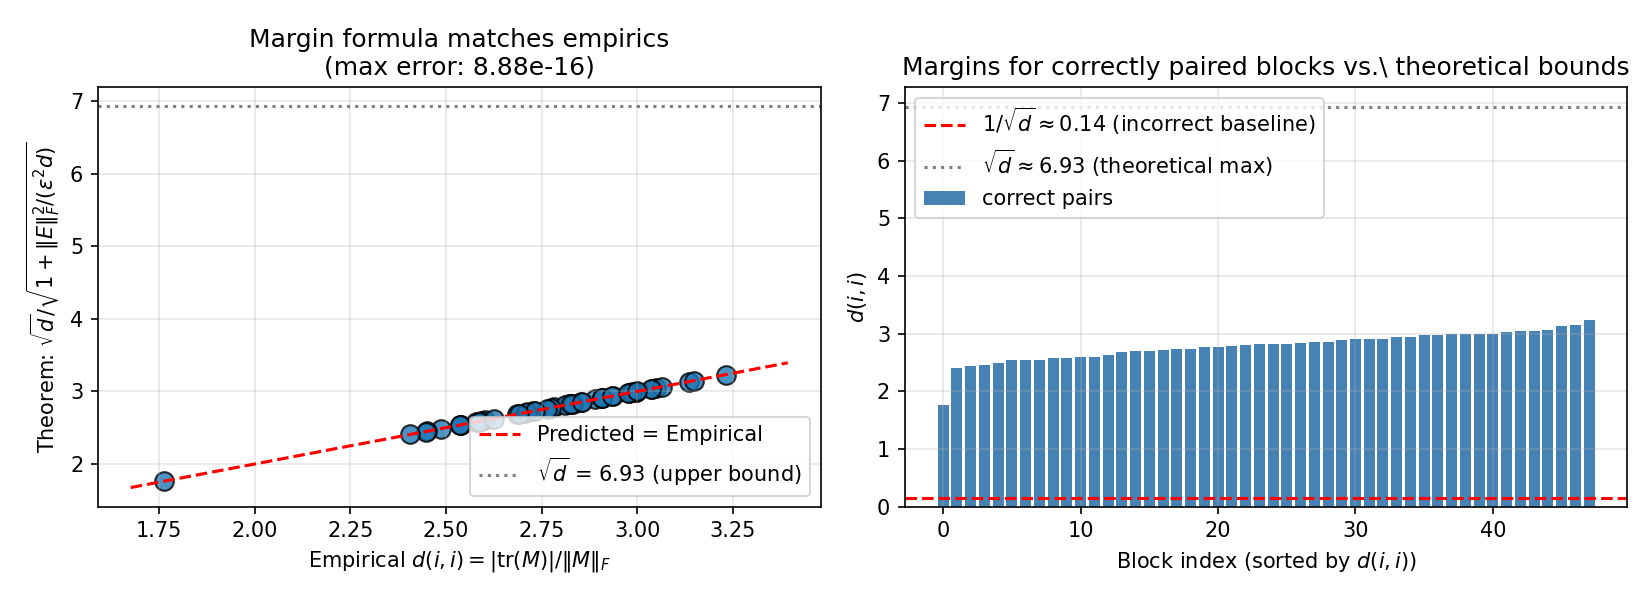
\includegraphics[width=\linewidth]{figures/fig_margin_theorem.png}
\caption{Proposition~\ref{prop:margin} reproduces the empirical margin
to floating-point precision. \emph{Left}: predicted $d(i,i)$ from the
formula vs.\ empirical $d(i,i)$ for all 48 correctly paired blocks of
Park's network. The points lie exactly on the diagonal (max abs.\
error $<10^{-15}$). The grey dotted line marks the upper bound
$\sqrt{d}\!\approx\!6.93$; correct pairs fall well below because of
off-diagonal energy $\|E\|_F>0$. \emph{Right}: sorted margins for
correct pairs (blue bars) sandwiched between the $1/\sqrt{d}$
incorrect-pair baseline (red dashed) and the theoretical upper bound
(grey dotted).}\label{fig:margin_theorem}
\end{figure}

\paragraph{Why a ratio beats raw Frobenius.} A natural alternative is
to pair by minimum $\|W_{\mathrm{out}}^{(j)} W_{\mathrm{in}}^{(i)}\|_F$
directly. On Park's puzzle, Hungarian on $\|M\|_F$ \emph{does} recover
all 48 pairs (it is the global optimum that saves it), but the absolute
margin
$\min_i \|M_{ii}\|_F - \max_{i\neq j} \|M_{ij}\|_F$
is \emph{negative}: $-0.452$. By contrast, for the diagonal-dominance
ratio the same margin is $+2.022$. The ratio normalizes away the
overall scale of $\|M\|_F$ (which varies across blocks for unrelated
reasons) and isolates the structural trace contribution that only
correctly paired products possess. This is the $\sqrt{d}$ factor in
Corollary~\ref{cor:worst} manifesting as a $\sim 4\times$ headroom on
the per-pair margin, and (because Hungarian's tolerance scales with
margin gap) the difference between fragile and robust pairing.

\subsection{Pairing Wall slope, from first principles}\label{sec:wall-theory}

Park~\cite[\S 5.1]{park2026} reports that earlier approaches stall at
MSE $\in[0.03, 0.5]$ when local search converges with a few wrong
pairings, but does not quantify the relationship. We give a
first-order prediction of the wall's slope in the small-mispair regime.

\begin{proposition}[Pairing Wall, linear regime]\label{prop:wall}
Let $f_\sigma$ be the network with ground-truth ordering and $k$
randomly chosen blocks repaired with random partners. Let
$\Delta r_{(k)}(x)$ denote the change in the residual contribution of
the $k$-th mispaired block. Under the first-order assumption that the
total deviation is the sum of per-block deviations (i.e., that
$\sum_k \Delta r_{(k)}$ is small relative to the residual stream norm,
so downstream blocks act linearly on the perturbation), the average
MSE satisfies
\[
  \overline{\mathrm{MSE}}(k) \;\approx\; k\cdot C,
  \qquad C \;=\; \mathbb{E}\!\left[\frac{\|W_{\mathrm{last}}\,\Delta r\|^2}{N}\right],
\]
where $\Delta r$ is the residual perturbation from a single random
mispair, evaluated on the input distribution.
\end{proposition}

\begin{proof}[Proof sketch]
Each mispaired block contributes $\Delta r_{(k)}(x)$ to the residual
stream. In the small-perturbation regime the downstream blocks are
$I + O(\varepsilon)$ in their Jacobians, so the perturbation passes
through to the output approximately linearly. The output deviation
from $f_\sigma(x)$ is $W_{\mathrm{last}} \sum_k \Delta r_{(k)}(x)$. Squaring
and averaging over $x\sim\mathcal{D}$:
$\mathbb{E}[(\hat y - y)^2] = \mathbb{E}\big[\|W_{\mathrm{last}}\sum_k \Delta r_{(k)}\|^2\big]/N$.
If mispairs are independent and identically distributed across blocks,
expectation is additive and yields $kC$.
\end{proof}

\paragraph{Numerical verification.} Computing $C$ directly from Park's
network via Monte Carlo (60 trials, one random pair-swap each, average
per-mispair MSE), we obtain $C \approx 0.0030$. The empirical fit
to $\overline{\mathrm{MSE}}(k)$ over $k\in[1,8]$ gives a slope of
$\approx 0.004$ (Section~\ref{sec:wall}, Fig.~\ref{fig:wall_theory}).
The first-order theory captures the slope to within $\sim 25\%$. The
remaining gap is the \emph{super-linear} second-order coupling between
mispairs, which becomes dominant for $k\gtrsim 12$ (the $k^{1.4}$
regime in Fig.~\ref{fig:wall}).

\begin{figure}[H]
\centering
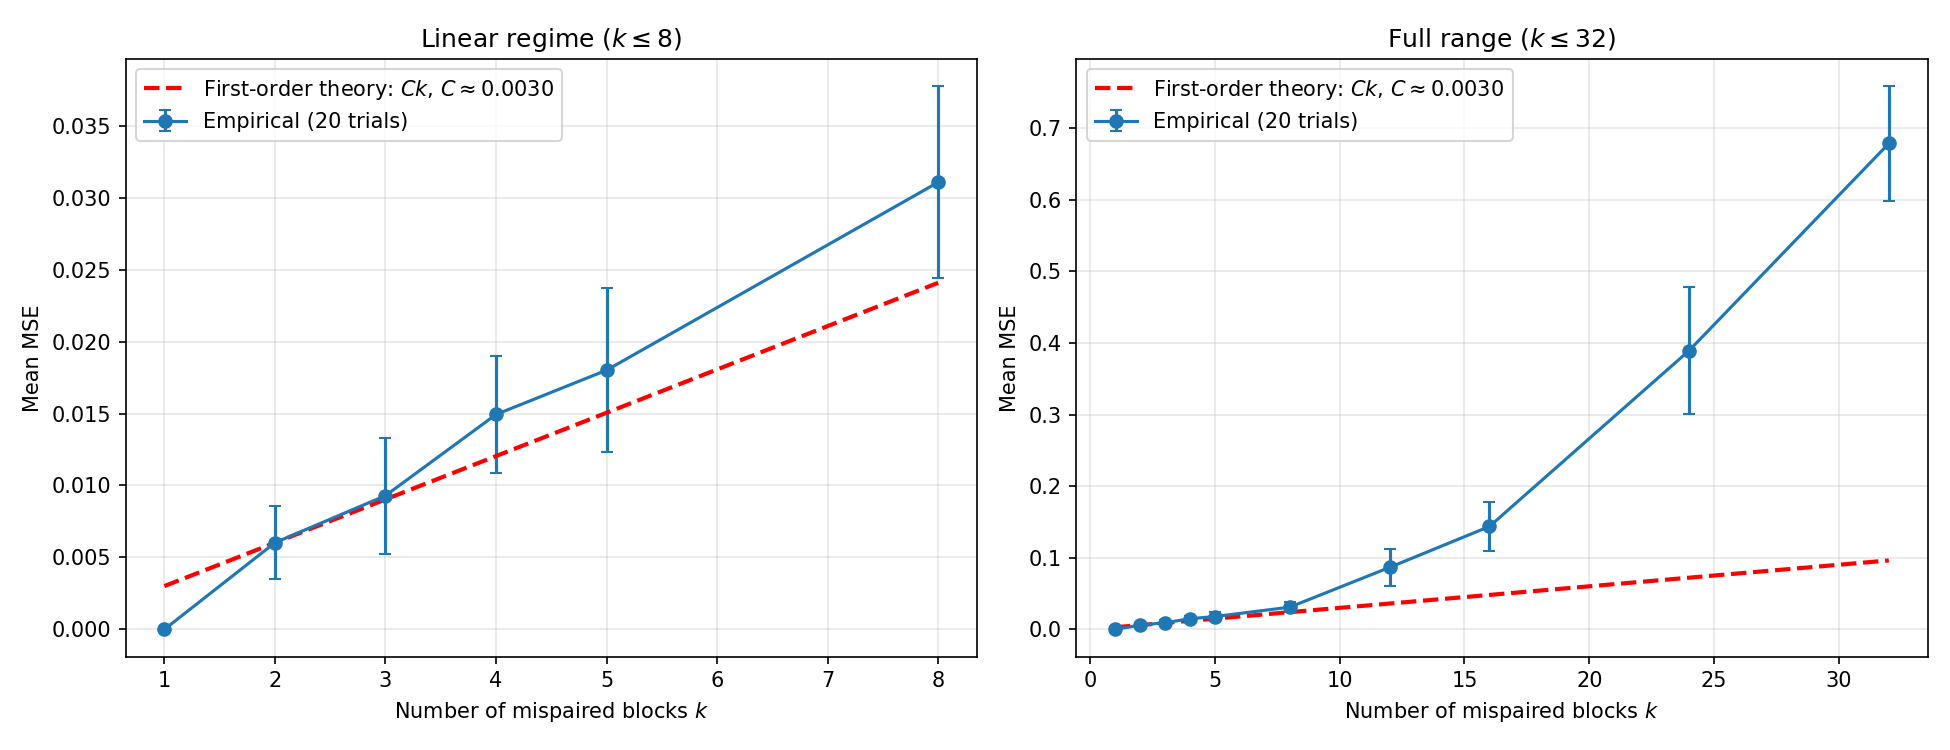
\includegraphics[width=\linewidth]{figures/fig_pairing_wall_theory.png}
\caption{Pairing Wall: empirical mean MSE (20 trials per $k$) with
$\pm\sigma$ error bars (blue), overlaid against the first-order
theoretical prediction $\overline{\mathrm{MSE}}(k)=Ck$ with
$C\!\approx\!0.0030$ from Proposition~\ref{prop:wall} (red dashed).
\emph{Left}: linear regime $k\leq 8$, where the agreement is tight.
\emph{Right}: full range $k\leq 32$, where second-order coupling
between simultaneous mispairs makes the curve grow super-linearly
($\propto k^{1.4}$).}\label{fig:wall_theory}
\end{figure}

\begin{remark}
Proposition~\ref{prop:wall} gives an operational diagnostic: if a
pipeline stalls at MSE $\mu$, the expected number of remaining mispairs
is $\hat k \approx \mu / C$. For Park's puzzle, MSE $=0.03$
suggests $\hat k\approx 10$ wrong pairings, broadly consistent with
where joint singular-value methods are reported to fail.
\end{remark}

\subsection{Null model: the signal requires training}\label{sec:nullmodel}

Proposition~\ref{prop:margin} assumes the trained decomposition
$M_{ii} = -\varepsilon I + E$ with $\varepsilon = |\mathrm{tr}(M_{ii})|/d > 0$.
For a randomly initialized network --- before any gradient steps ---
there is no mechanism producing this negative-diagonal structure: the
sign of $\mathrm{tr}(W_{\mathrm{out}}^{(i)} W_{\mathrm{in}}^{(i)})$ is
not constrained, and correctly paired and incorrectly paired products
are drawn from the same distribution. Corollary~\ref{cor:worst} then
applies to \emph{every} entry of the score matrix, predicting
$\mathbb{E}[d(i,j)] \to 1/\sqrt{d}$ uniformly.

\begin{corollary}[Null model]\label{cor:null}
Suppose $W_{\mathrm{in}}^{(i)}$ and $W_{\mathrm{out}}^{(j)}$ are
independent random matrices with i.i.d.\ zero-mean entries, with no
training-induced coupling between corresponding indices. Then for every
$(i,j)$ (including $i=j$), $d(i,j)$ has the same expectation
$\mathbb{E}[d(i,j)] = 1/\sqrt{d} + o(1)$, and Hungarian pairing on
$-d$ recovers correct pairs at chance rate $1/D$ in expectation.
\end{corollary}

\paragraph{Empirical verification: the training trajectory.} We
instantiate Corollary~\ref{cor:null} on Park's exact shape (depth $48$,
hidden $96$), Kaiming-initialized and never trained: pair accuracy is
$6.25\%$ (chance is $1/D = 2.08\%$; Hungarian over a noisy matrix
biases upward but stays close to chance), pair separation is $-0.42$,
and the correct-pair and incorrect-pair score means are
\emph{statistically indistinguishable} ($0.121$ vs.\ $0.114$). On the
trained Jane Street network, aligned to its recovered pairing, those
two means separate by a factor of $\sim 21\times$ and Hungarian
recovers all $48/48$ pairs.

To make the temporal dependence explicit we then train a single
ResNet ($D{=}24$, $h{=}64$) from scratch and snapshot the pairing
matrix at five points along the trajectory. Figure~\ref{fig:nullmodel}
shows the full picture in one shot.

\begin{figure}[H]
\centering
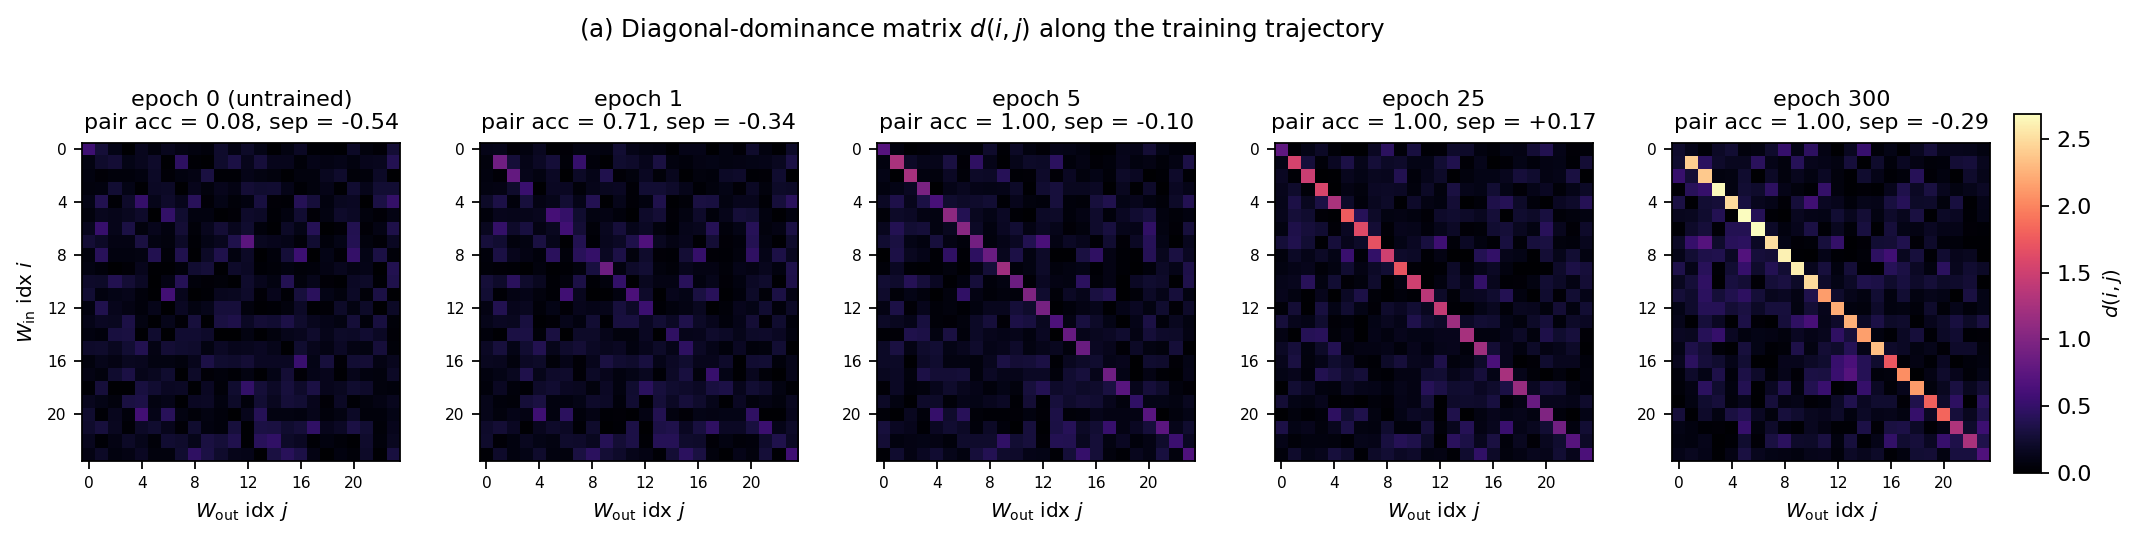
\includegraphics[width=\linewidth]{figures/fig_null_a_heatmaps.png}
\caption{\textbf{(a)} Diagonal-dominance matrix $d(i,j)$ at five
training stages of a single $24$-block ResNet. At initialization
there is no visible diagonal; by epoch $5$ the diagonal is fully
separated. The bright off-diagonal entries at epoch $300$ are not
structural --- the diagonal still dominates each row.}\label{fig:null_a}
\end{figure}

\begin{figure}[H]
\centering
\begin{subfigure}{0.48\linewidth}
  \centering
  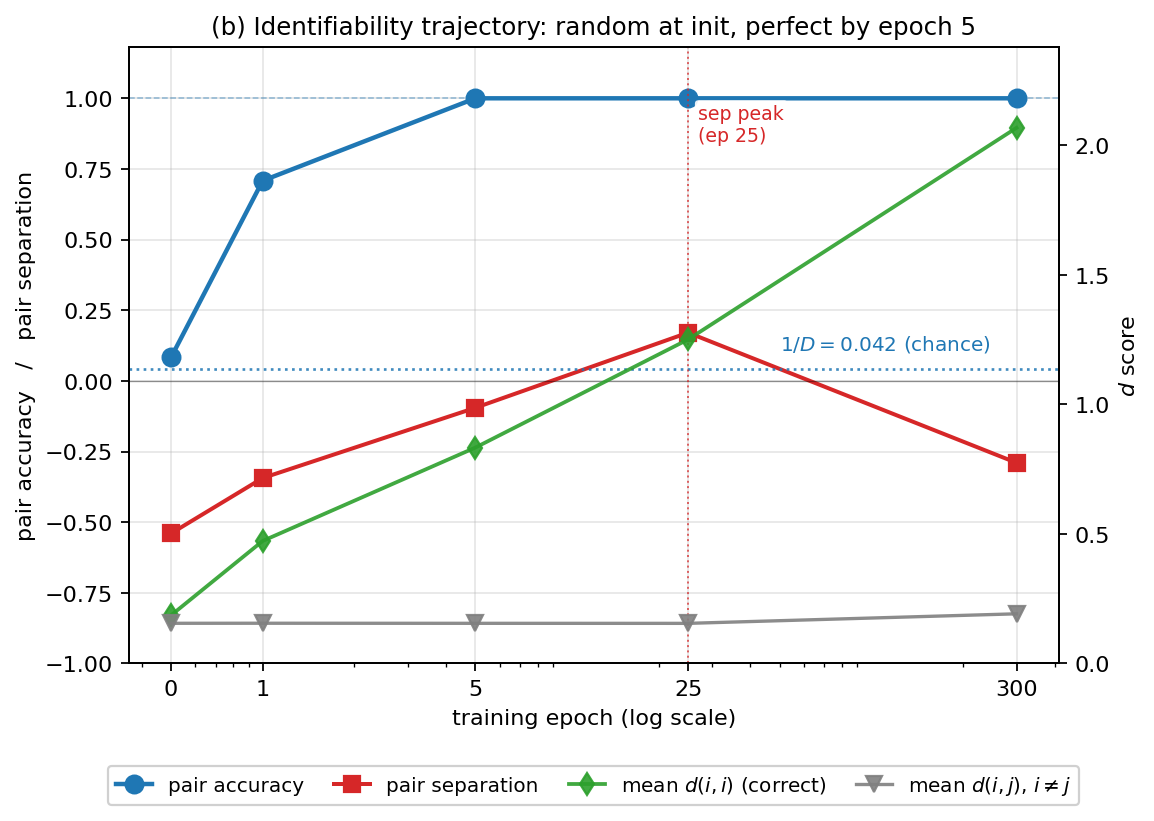
\includegraphics[width=\linewidth]{figures/fig_null_b_trajectory.png}
  \caption{Identifiability trajectory. Pair accuracy jumps from chance
  ($0.08$ at epoch $0$, with $1/D=0.042$) to $1.00$ by epoch $5$. Mean
  correct-pair score (right axis) rises monotonically from $0.19$ to
  $2.07$ while the mean incorrect-pair score stays flat at $\approx
  0.16$. Pair separation peaks at epoch $25$ and drifts back to $-0.29$
  at epoch $300$ even as pair accuracy stays perfect.}\label{fig:null_b}
\end{subfigure}\hfill
\begin{subfigure}{0.48\linewidth}
  \centering
  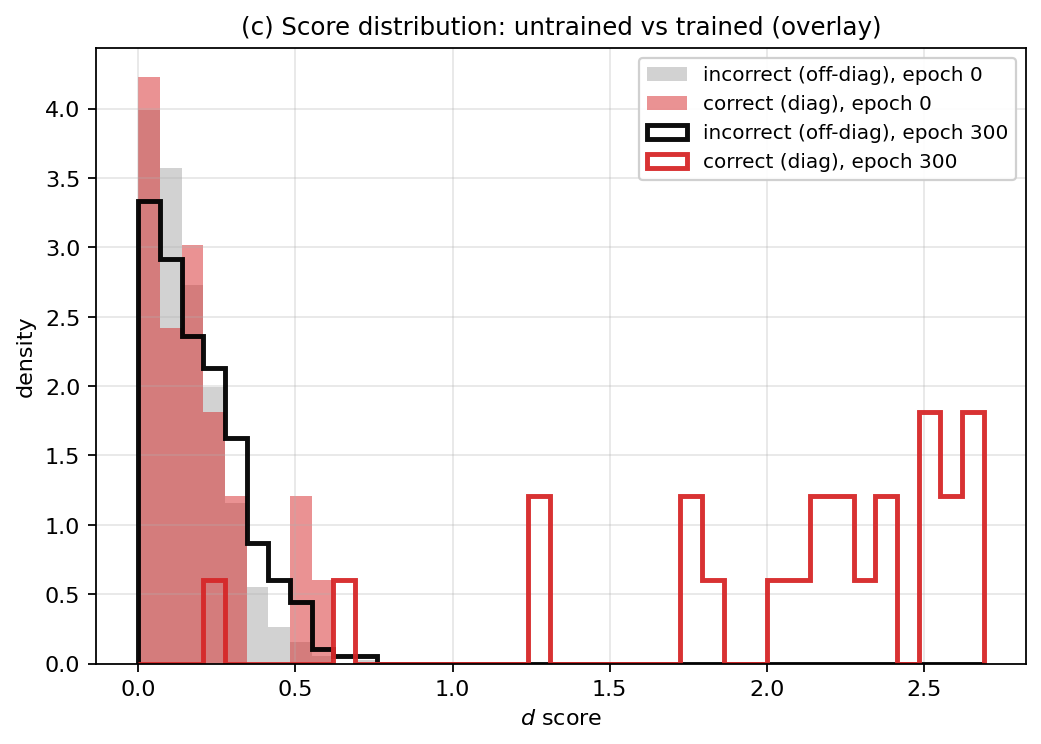
\includegraphics[width=\linewidth]{figures/fig_null_c_histograms.png}
  \caption{Score distribution overlay. At epoch $0$ the correct (filled
  red) and incorrect (filled gray) score densities are nearly identical.
  After $300$ epochs the correct-pair scores (red outline) move out to
  $1.3$--$2.7$ while the incorrect-pair scores (black outline) stay
  pinned near zero.}\label{fig:null_c}
\end{subfigure}

\vspace{0.6em}
\begin{subfigure}{0.7\linewidth}
  \centering
  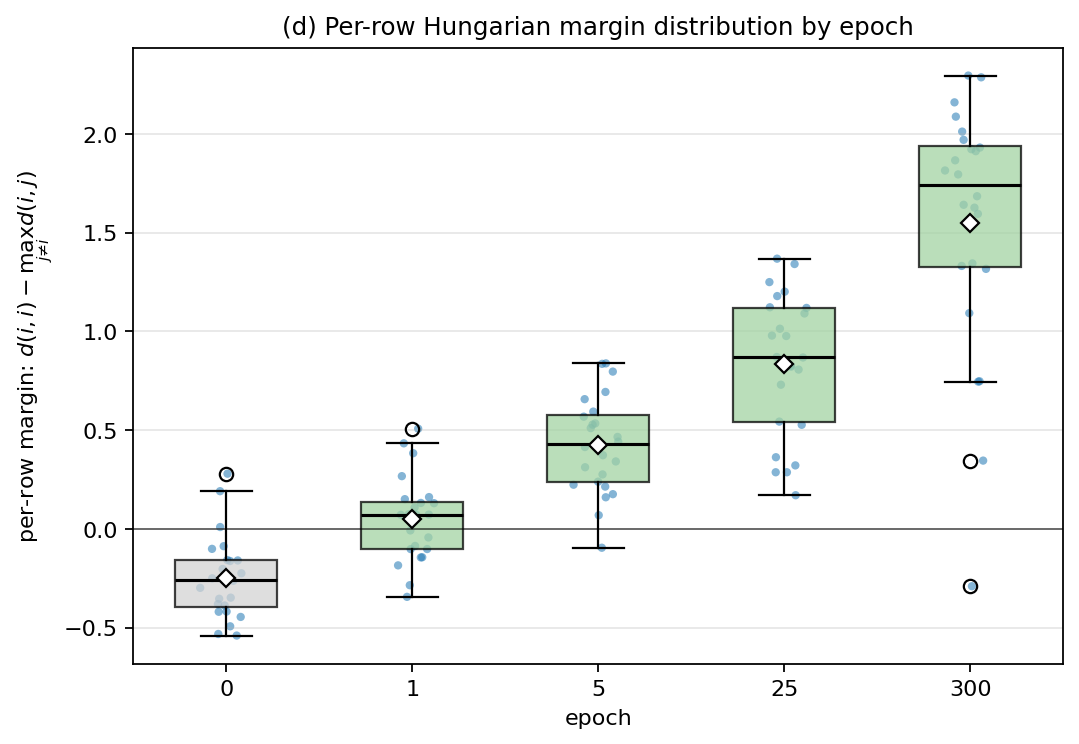
\includegraphics[width=\linewidth]{figures/fig_null_d_margins.png}
  \caption{Per-row Hungarian margin distribution. Even when the
  \emph{global} pair separation $\min_i\big(d(i,i) - \max_{j\neq
  i}d(i,j)\big)$ is negative, the \emph{per-row} margins are positive
  at every epoch from $5$ onward --- which is exactly why Hungarian
  recovers $100\%$ of pairs there, the rescue described in
  Obs.~\ref{obs:fro}.}\label{fig:null_d}
\end{subfigure}
\caption{\textbf{Null model deep dive (continued).}}\label{fig:nullmodel}
\end{figure}

\paragraph{What this rules out.} The figure rules out three obvious
``trivial'' alternative explanations a skeptical reader could propose:
\textbf{(a)} that diagonal dominance is an artifact of compatible
matrix shapes (it isn't: the untrained matrices have exactly the
shapes used in the puzzle yet produce a uniform score matrix);
\textbf{(b)} that the residual connection is what creates the signal
(it doesn't: a fresh residual network with no training shows no
diagonal); \textbf{(c)} that the signal could be present at any
nontrivial loss level (it isn't: at epoch $0$ the train loss is $10.2$
and the matrix is featureless; the diagonal sharpens monotonically as
loss decreases). The signal is therefore not topological or
distributional but a \emph{learned} property, in exact agreement with
the dynamic-isometry mechanism behind Proposition~\ref{prop:margin}.
As a bonus, the trajectory recapitulates the non-monotonic
identifiability of Observation~\ref{obs:nonmono} on a single network:
pair separation peaks at epoch $25$ ($+0.17$) and drifts back to
$-0.29$ by epoch $300$ even as pair accuracy stays at $1.00$ and the
training loss continues to fall.



\section{Anatomy of the Pairing Signal}\label{sec:pair-anatomy}
We begin with a forensic look at the reference 48-block network. Figure~\ref{fig:matrix}
visualizes the $48\times 48$ diagonal-dominance matrix in true depth
order: a bright diagonal stands out against an unstructured background,
which is what makes the puzzle tractable. The worst-case correct-pair
score is $1.76$ and best-case incorrect-pair score is $0.58$, giving a
hard separation of $1.18$.

\begin{figure}[H]
\centering
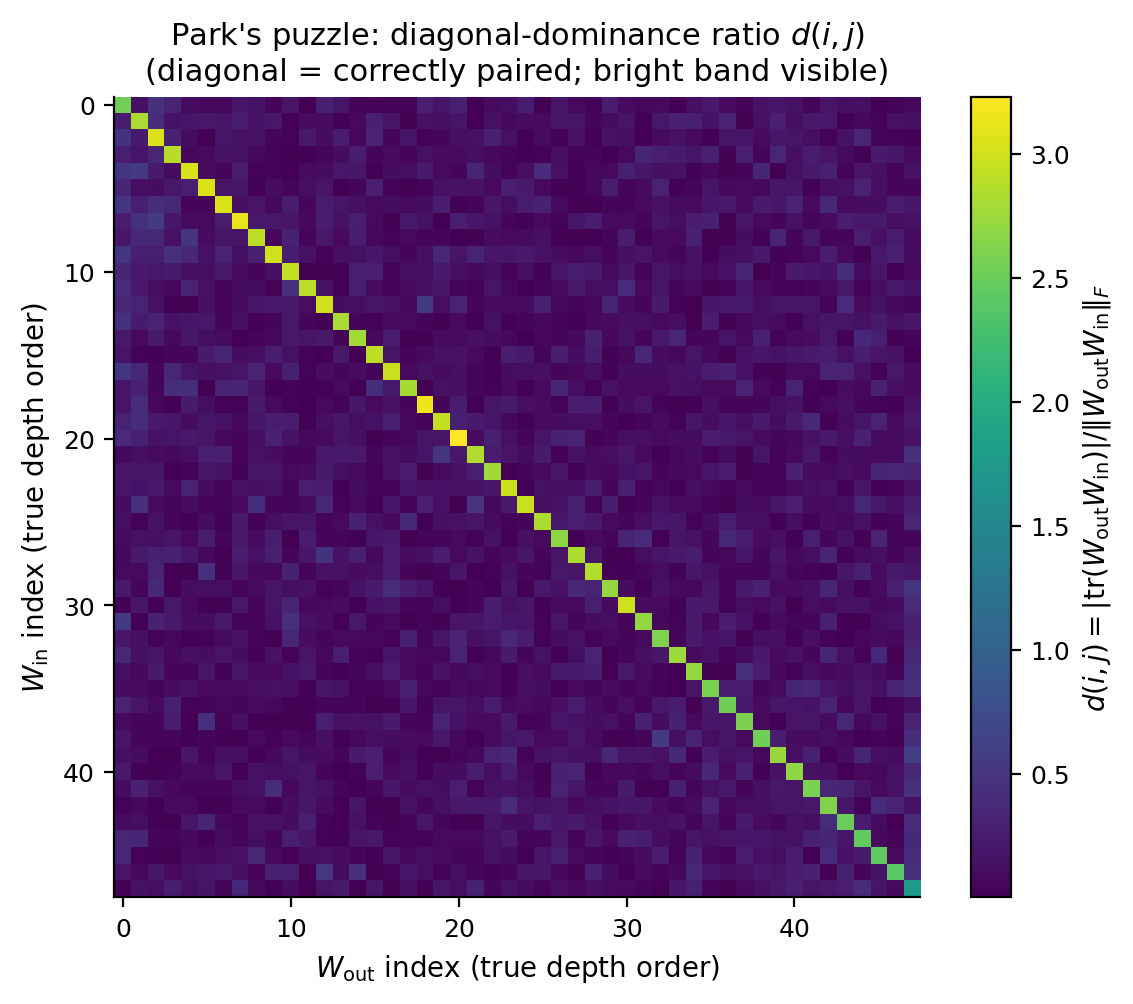
\includegraphics[width=0.6\linewidth]{figures/fig_pairing_matrix_park.png}
\caption{Diagonal-dominance ratio matrix $d(i,j)$ for Park's puzzle network,
rows and columns reordered into true depth order. The bright diagonal is
the training signal that \eqref{eq:diag} exploits.}\label{fig:matrix}
\end{figure}

\subsection{Why the ratio works in practice: a 250$\times$ per-row margin}

Section~\ref{sec:theory} gives the exact margin formula
(Proposition~\ref{prop:margin}) and the asymptotic $\sqrt{d}$ headroom
(Corollary~\ref{cor:worst}). Here we report the practical consequence:
on Park's puzzle network, of four candidate pairing metrics evaluated
against the ground truth (Fig.~\ref{fig:metrics}), only two achieve
$48/48$ recovery, and the difference in robustness is dramatic.

\begin{figure}[H]
\centering
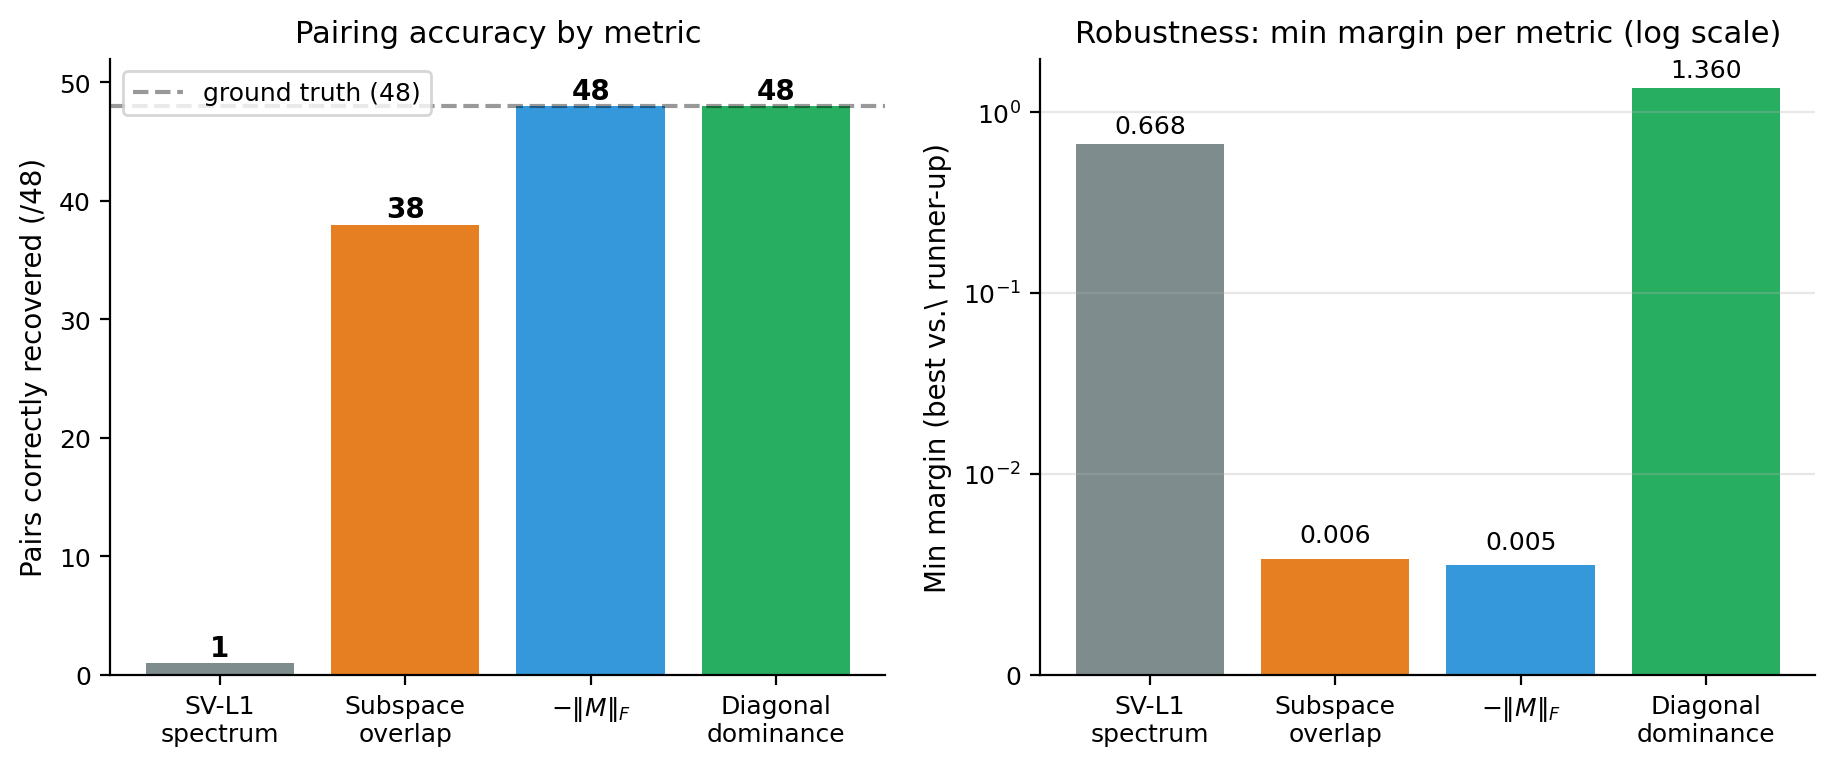
\includegraphics[width=\linewidth]{figures/fig_metric_comparison.png}
\caption{Four candidate pairing metrics, scored against the ground-truth
permutation. \emph{Left}: number of correctly recovered pairs (out of 48).
\emph{Right}: per-row Hungarian margin (best vs.\ runner-up cost),
log-scaled. Two metrics achieve $48/48$ but with margins differing by
$250\times$.}\label{fig:metrics}
\end{figure}

\begin{observation}[Two metrics pair perfectly; only one is robust]\label{obs:fro}
The bare Frobenius product $-\|W_{\mathrm{out}}^{(j)} W_{\mathrm{in}}^{(i)}\|_F$
also recovers all $48$ correct pairs on Park's puzzle --- but with a
minimum per-row margin of $0.005$, versus $1.36$ for diagonal
dominance: a $250\times$ gap. Globally,
$\min_i \|M_{ii}\|_F - \max_{i\neq j} \|M_{ij}\|_F = -0.452$ is in fact
\emph{negative}: Frobenius cannot separate correct from incorrect pairs
without Hungarian's global-optimum rescue.
\end{observation}

The mechanism is exactly Proposition~\ref{prop:margin}: $\|M\|_F$ for
correct pairs is dominated by $\varepsilon^2 d + \|E\|_F^2$, while
$\|M\|_F$ for incorrect pairs is $O(d h \sigma_{\mathrm{out}}^2\sigma_{\mathrm{in}}^2)$;
these two scales overlap because they have no clean common
denominator. Dividing by $\|M\|_F$ kills the scale and isolates the
$\varepsilon$-trace contribution.

\subsection{Subspace overlap: the natural alternative that fails}

A second natural candidate, also worth highlighting, is subspace overlap
via principal angles: paired $(W_{\mathrm{in}}, W_{\mathrm{out}})$ should
share the 48-dim subspace of the 96-dim hidden representation they
communicate through. This is the same machinery as
SVCCA~\cite{raghu2017svcca} and CKA~\cite{kornblith2019cka}, standard
tools for representational similarity.

It works partially --- $38/48$ correct pairs on Park's network --- but
not enough for exact reassembly. The ten failures reveal something
useful: multiple blocks operate on \emph{nearly identical} 48-dim
subspaces of the hidden space, yet pair with different partners during
training. Subspace alignment is a necessary but not sufficient signal:
two blocks can read from the same subspace and still be unrelated. The
diagonal structure of $M_{\pi^\star(i),i}$ captures the
\emph{interaction} of $W_{\mathrm{in}}$ and $W_{\mathrm{out}}$, not just
their geometric overlap, and this distinction is what makes
\eqref{eq:diag} succeed where subspace overlap stalls.

\subsection{The Pairing Wall: MSE as a function of pairing errors}\label{sec:wall}

Several earlier approaches to this puzzle (singular-value matching,
joint simulated annealing, etc.) plateau at MSE $\in [0.03, 0.5]$.
Park notes this informally~\cite[Sec.~5.1]{park2026}. We characterize
it directly: starting from the exact solution and the true ordering,
randomly permute the $W_{\mathrm{out}}$ partners of $k$ blocks (without
fixed points), and average MSE over $20$ trials.

\begin{figure}[H]
\centering
\begin{subfigure}[t]{0.48\linewidth}
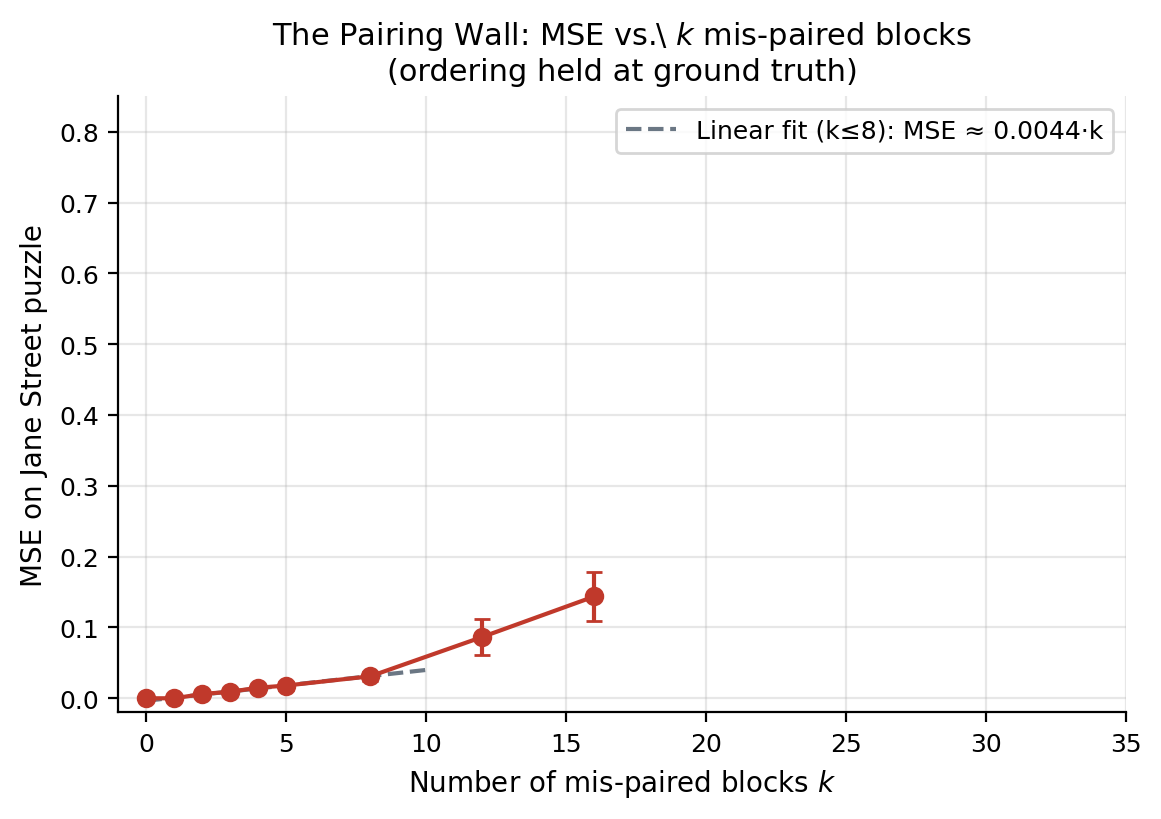
\includegraphics[width=\linewidth]{figures/fig_pairing_wall.png}
\caption{Linear scale, $k\leq 32$.}
\end{subfigure}\hfill
\begin{subfigure}[t]{0.48\linewidth}
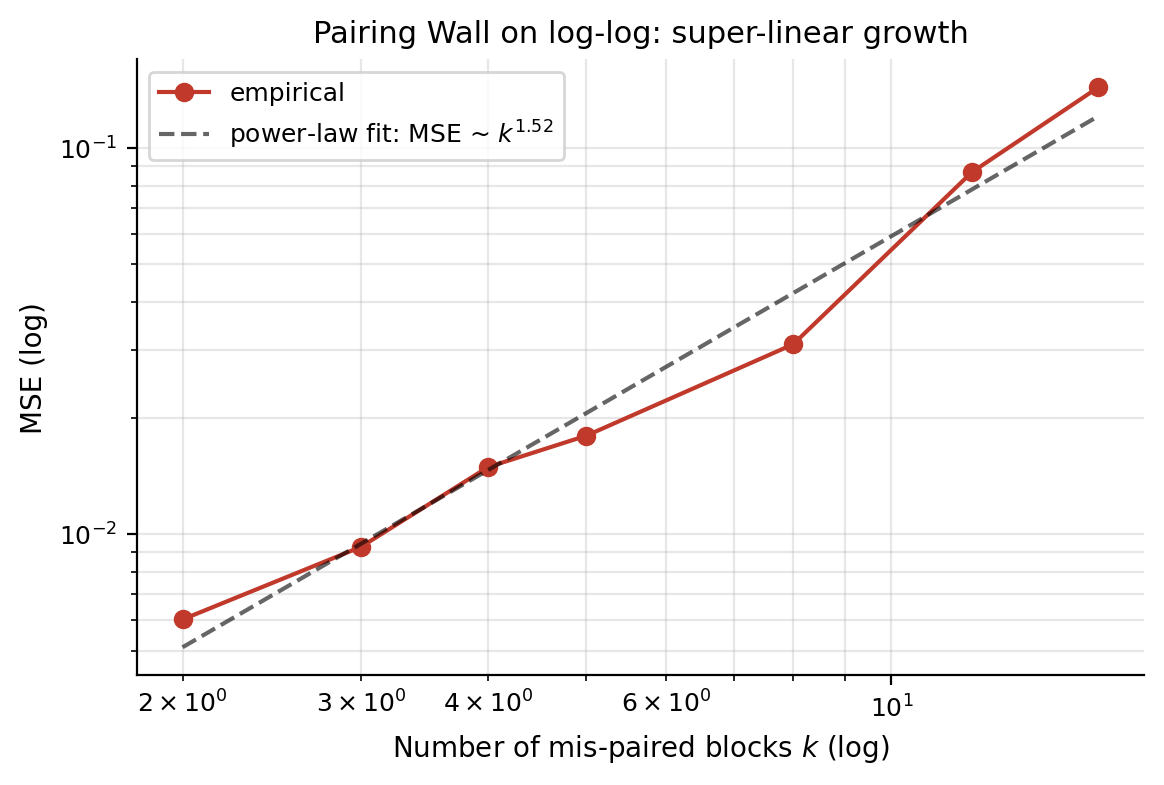
\includegraphics[width=\linewidth]{figures/fig_pairing_wall_loglog.png}
\caption{Log--log, $k\in[2, 16]$.}
\end{subfigure}
\caption{The Pairing Wall: MSE versus number of mis-paired blocks
(ordering held at ground truth). Two regimes: roughly linear for
$k\lesssim 8$ with slope $\approx 0.004$; super-linear thereafter with
log-log slope $\approx 1.4$.}
\label{fig:wall}
\end{figure}

\begin{observation}[Two regimes of the wall]\label{obs:wall}
$\overline{\mathrm{MSE}}(k)$ exhibits two regimes:
\textbf{(i)}~linear for $k\lesssim 8$, with slope $\approx 0.004$
per mis-pair --- so one wrong pair already costs MSE $\approx 0.003$;
\textbf{(ii)}~super-linear for $k\gtrsim 12$, MSE $\propto k^{1.4}$, with
the variance growing as some derangements align with the flow of
information and others do not.
\end{observation}

This is the diagnostic missing from earlier approaches. If local search
stalls at MSE $\in [0.005, 0.05]$, the pairing has approximately
$2$--$10$ wrong pairs; reordering will not help and the pairing step
should be revisited.

\subsection{Pairing transfers to our trained ResNets}

\begin{figure}[H]
\centering
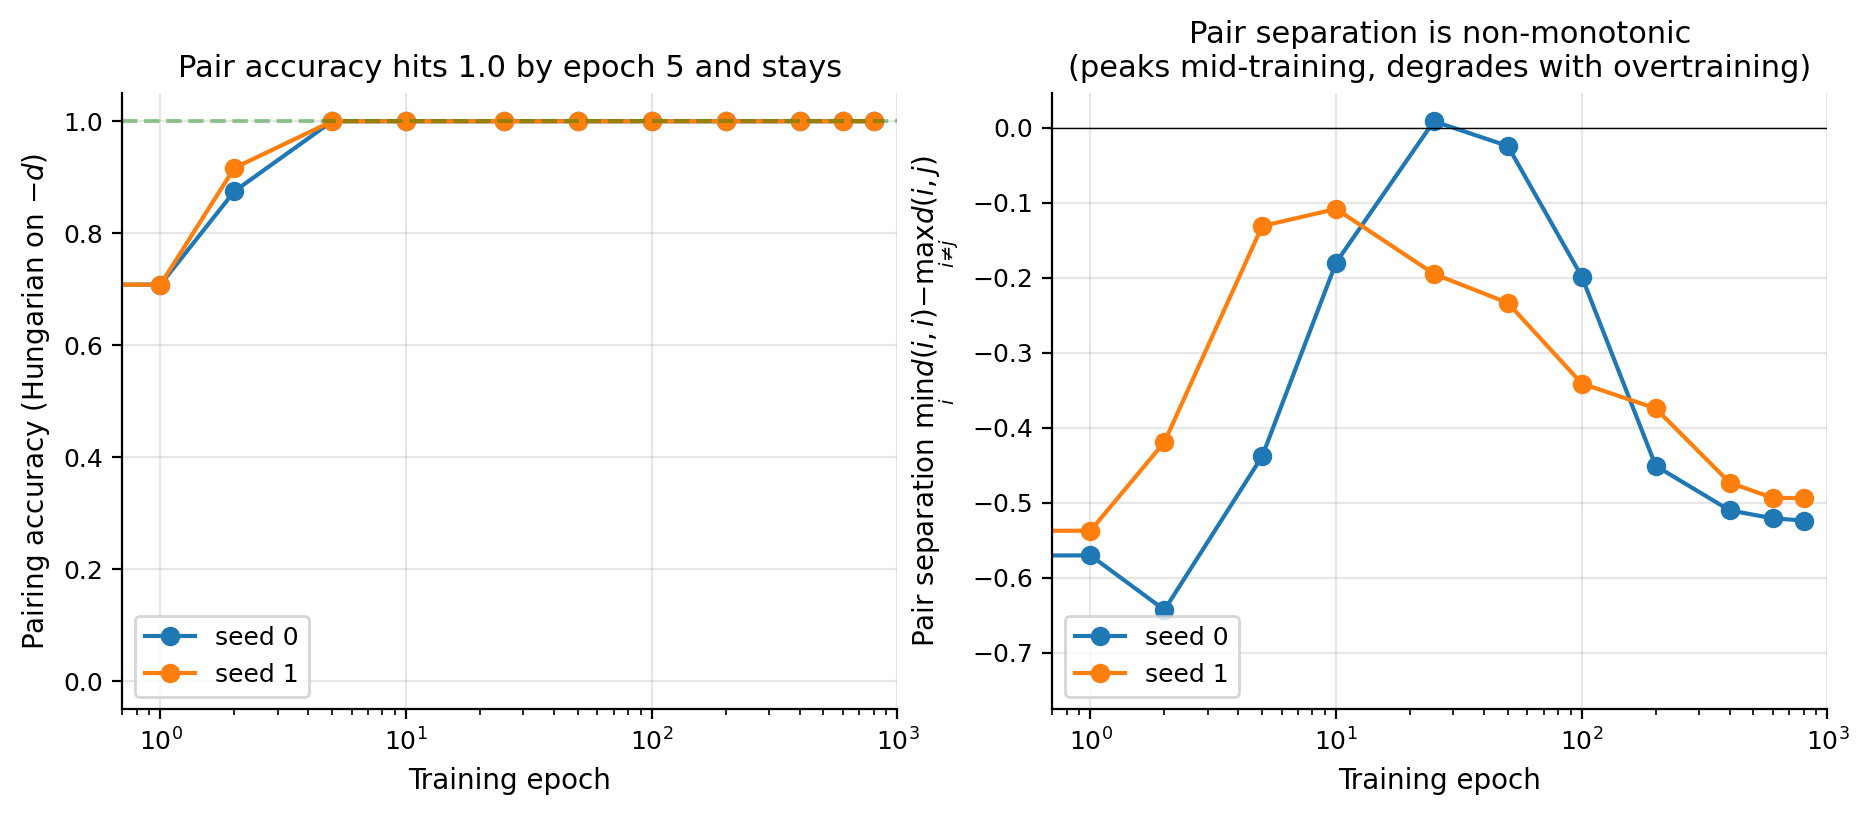
\includegraphics[width=\linewidth]{figures/fig_pair_acc_sep.png}
\caption{Pair accuracy (\emph{left}) and pair separation (\emph{right})
across training in a 24-block ResNet, two seeds. Pair accuracy reaches
1.0 by epoch 5--10 and stays. Separation is mostly negative, yet
Hungarian recovers the identity assignment: it is the global optimum of
the sum, not per-row dominance, that drives accuracy.}\label{fig:pair_acc_sep}
\end{figure}

\begin{observation}[Pairing is easy after little training]\label{obs:pair-gen}
On our 24-block synthetic ResNets, diagonal-dominance Hungarian achieves
$100\%$ pair accuracy by training epoch $5$ in every seed we tested,
despite negative per-row separation. The threshold is similar across
depths $\{8, 16, 24, 32\}$ in our wider sweep.
\end{observation}

Park's puzzle network exhibits hard positive separation ($+1.18$); ours
never do, yet Hungarian still matches perfectly. The diagonal-dominance
signal is meaningfully weaker on our networks than on Park's, but the
\emph{global} bipartite-matching optimum tolerates this weakness. This
is a useful generalization in its own right: the signal does not need to
be hard-separated for the method to succeed, only consistent enough that
the optimum permutation is unique.

\subsection{Generalization across the sweep}

Figure~\ref{fig:sweep_summary} extends the picture from one
configuration to the full sweep: $4$ architectures
$\times 3$ seeds $\times \sim 10$ training checkpoints
($\approx 100$ rows total). Pair accuracy reaches and holds at $1.0$
for almost every configuration after $\leq 25$ epochs of training. Pair
separation hovers below zero in the majority of configurations
(Hungarian rescue at work) but visibly trends \emph{up} during the
early training and then \emph{down} again as the network continues to
train --- the non-monotonic behaviour we will quantify in
Section~\ref{sec:order-anatomy}. The sign-flipping of $\rho$ relative
to Park is visible immediately: every synthetic configuration ends
with $\rho<0$, while Park's $\rho=+0.99$.

\begin{figure}[H]
\centering
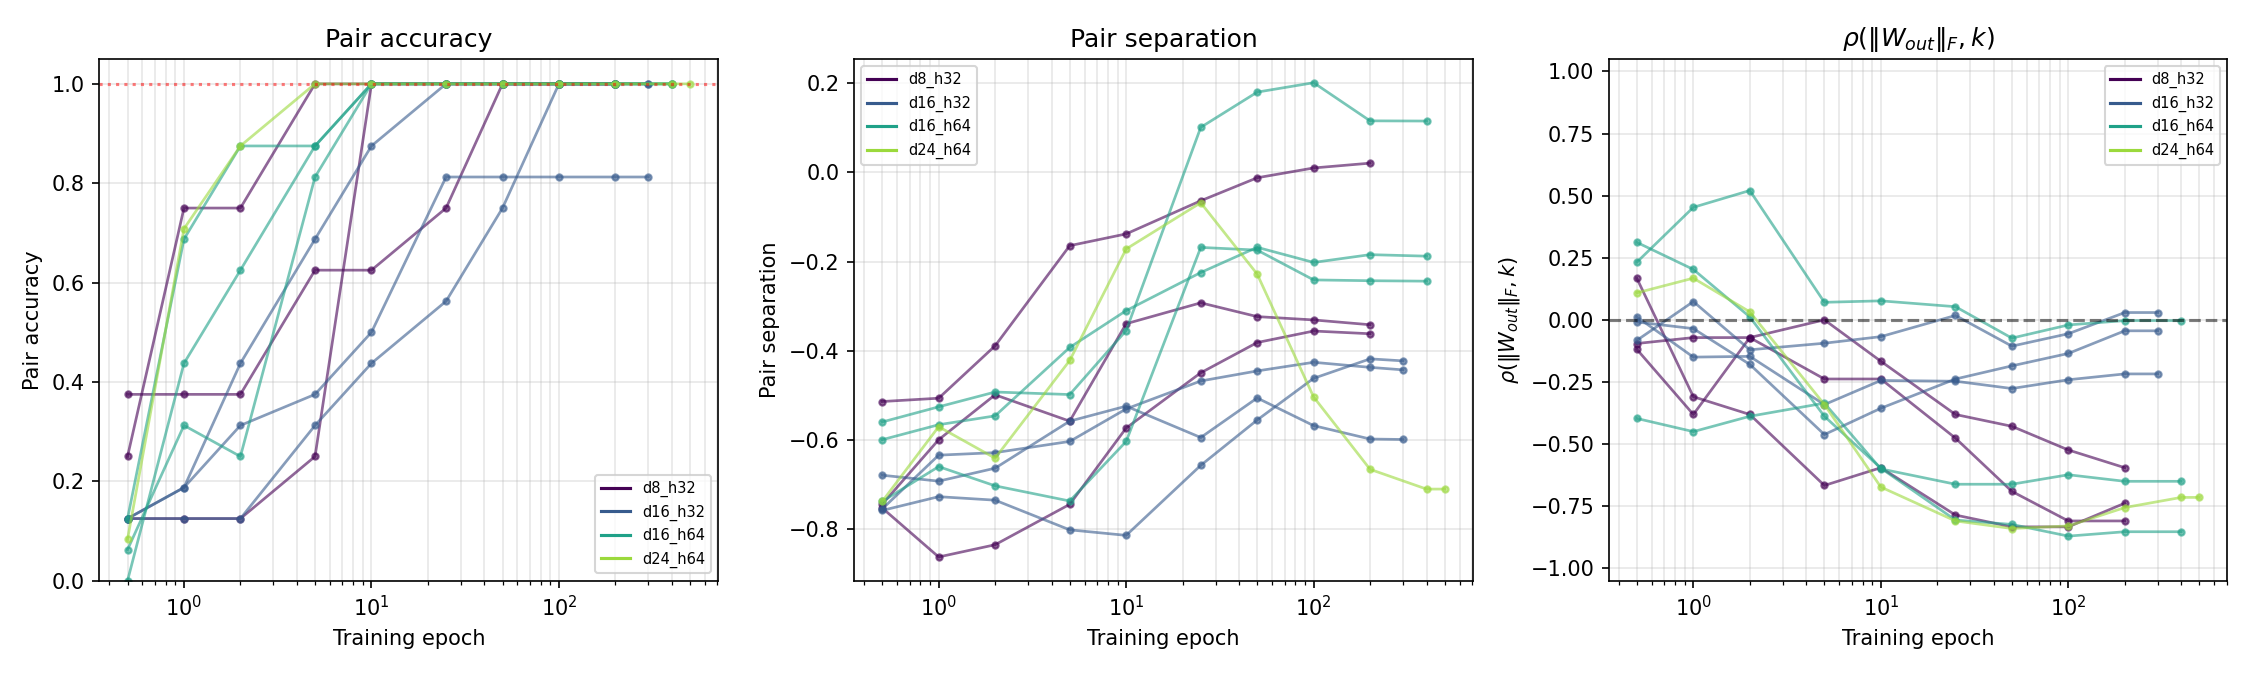
\includegraphics[width=\linewidth]{figures/fig_sweep_summary.png}
\caption{Pair accuracy, pair separation, and sort-direction
$\rho(\|W_{\mathrm{out}}\|_F, k)$ across training for four configurations
$\times$ three seeds. Pair accuracy reaches 1.0 quickly and stays.
Separation is mostly negative, with mid-training peaks visible in the
depth-16, width-64 configuration. $\rho$ is consistently negative on
our synthetic networks, opposite to the $+0.99$ measured on the
puzzle reference.}\label{fig:sweep_summary}
\end{figure}

% ====================================================================
\section{Anatomy of the Ordering Signal}\label{sec:order-anatomy}

\subsection{$\|W_{\mathrm{out}}\|_F$ as depth proxy on Park's network}

\begin{figure}[H]
\centering
\begin{subfigure}[t]{0.48\linewidth}
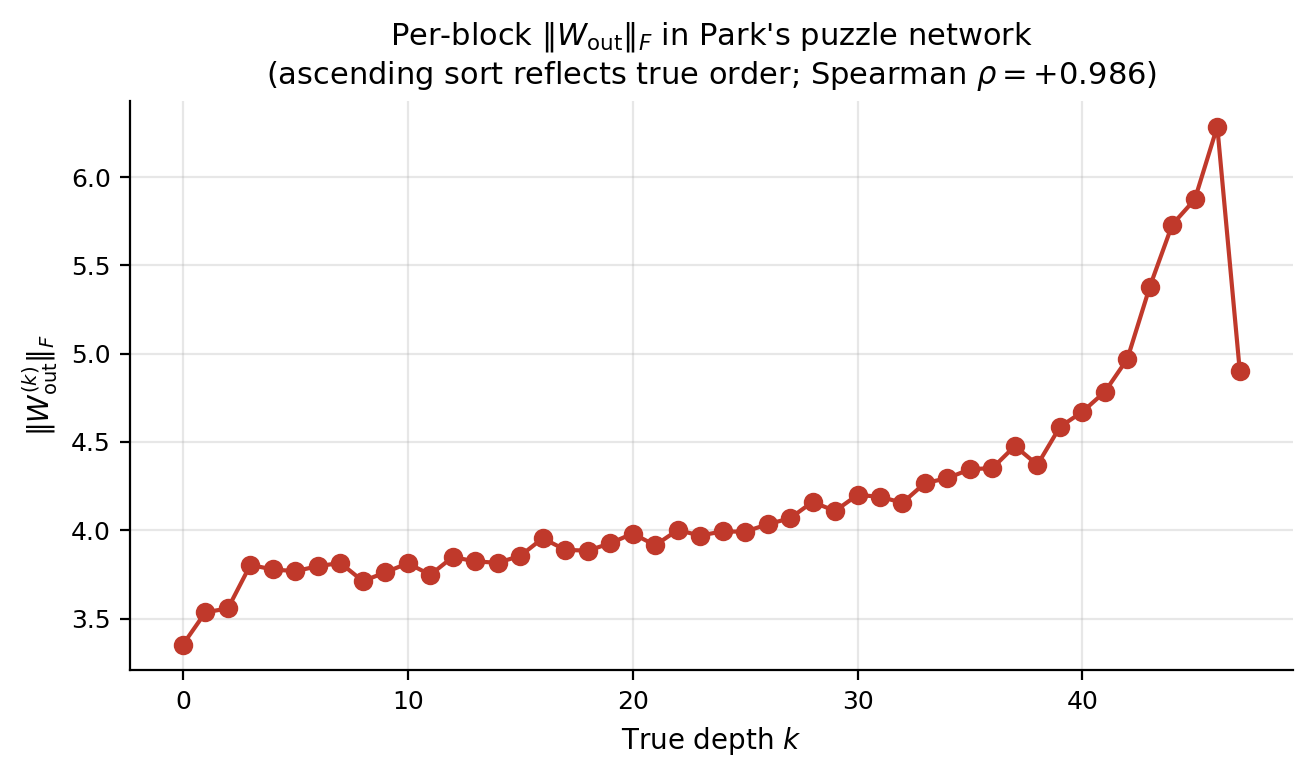
\includegraphics[width=\linewidth]{figures/fig_park_wout_per_block.png}
\caption{$\|W_{\mathrm{out}}^{(k)}\|_F$ vs.\ true depth $k$.}
\end{subfigure}\hfill
\begin{subfigure}[t]{0.48\linewidth}
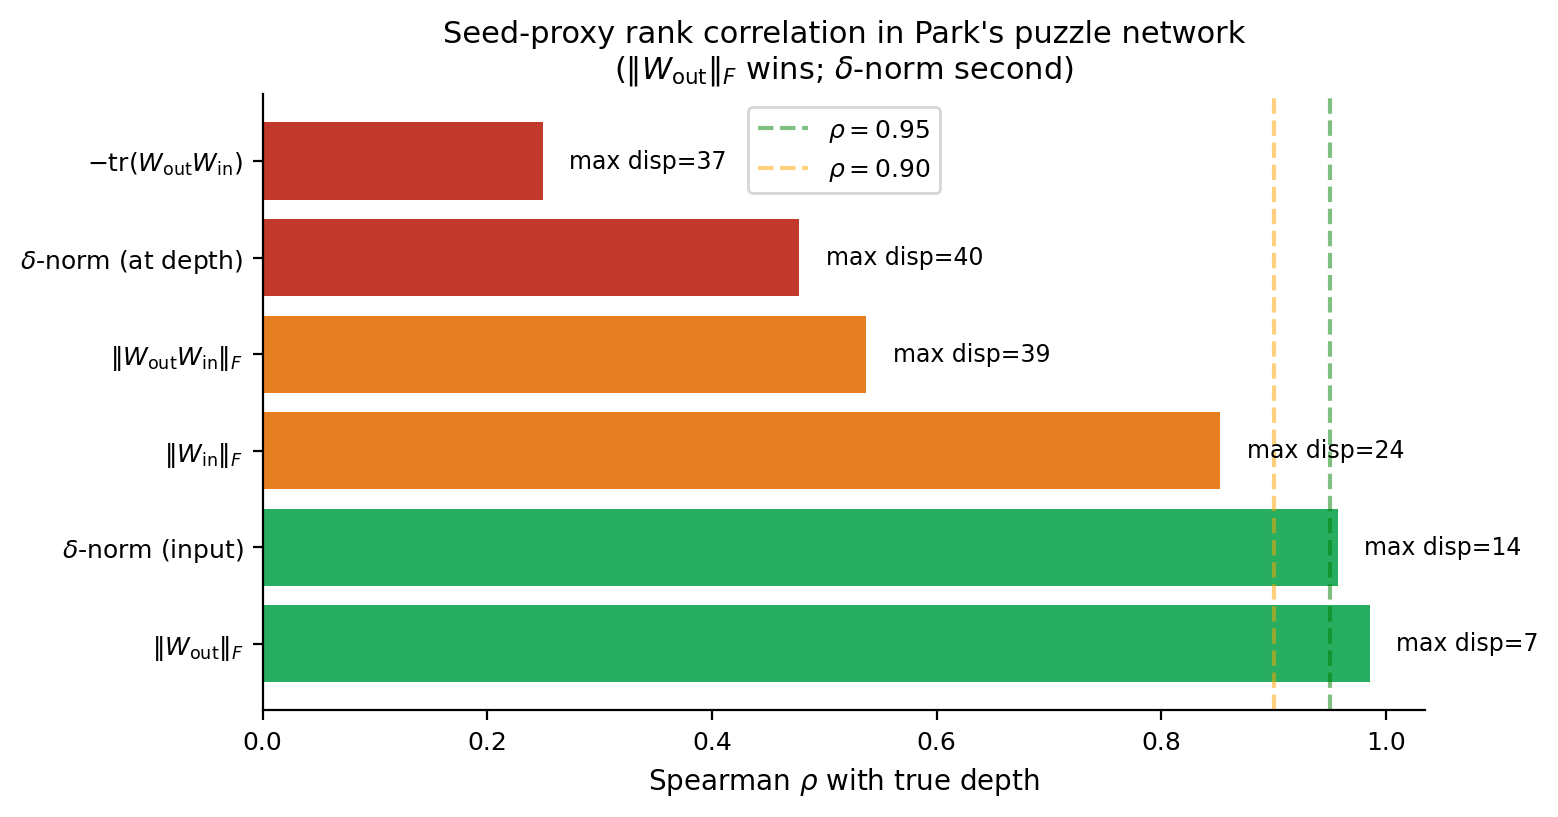
\includegraphics[width=\linewidth]{figures/fig_seed_rho.png}
\caption{Rank correlation of six seed proxies with true depth.}
\end{subfigure}
\caption{Park's puzzle network: $\|W_{\mathrm{out}}\|_F$ rises
monotonically with true depth (Spearman $\rho=+0.986$), and dominates the
five other natural proxies on both rank correlation and max
displacement.}\label{fig:park_seed}
\end{figure}

\paragraph{This resolves Park's Sec.~6.3 open question.} Park asks why
$\|W_{\mathrm{out}}\|_F$ as a seed converges \emph{faster} than
$\delta$-norm despite a \emph{worse} initial MSE. The answer we find is
that bubble-sort speed is governed by Kendall-tau distance to the truth
(i.e., inversion count), not by initial MSE.
$\|W_{\mathrm{out}}\|_F$ has fewer inversions to fix even though its MSE
starts higher: mean rank displacement is $1.54$ versus $2.79$ for
$\delta$-norm at the input. The bubble-sort budget per round is
linear in inversions, so fewer inversions $\Rightarrow$ faster
convergence.

\subsection{The proxy is not universal: sign flips on our networks}

\begin{figure}[H]
\centering
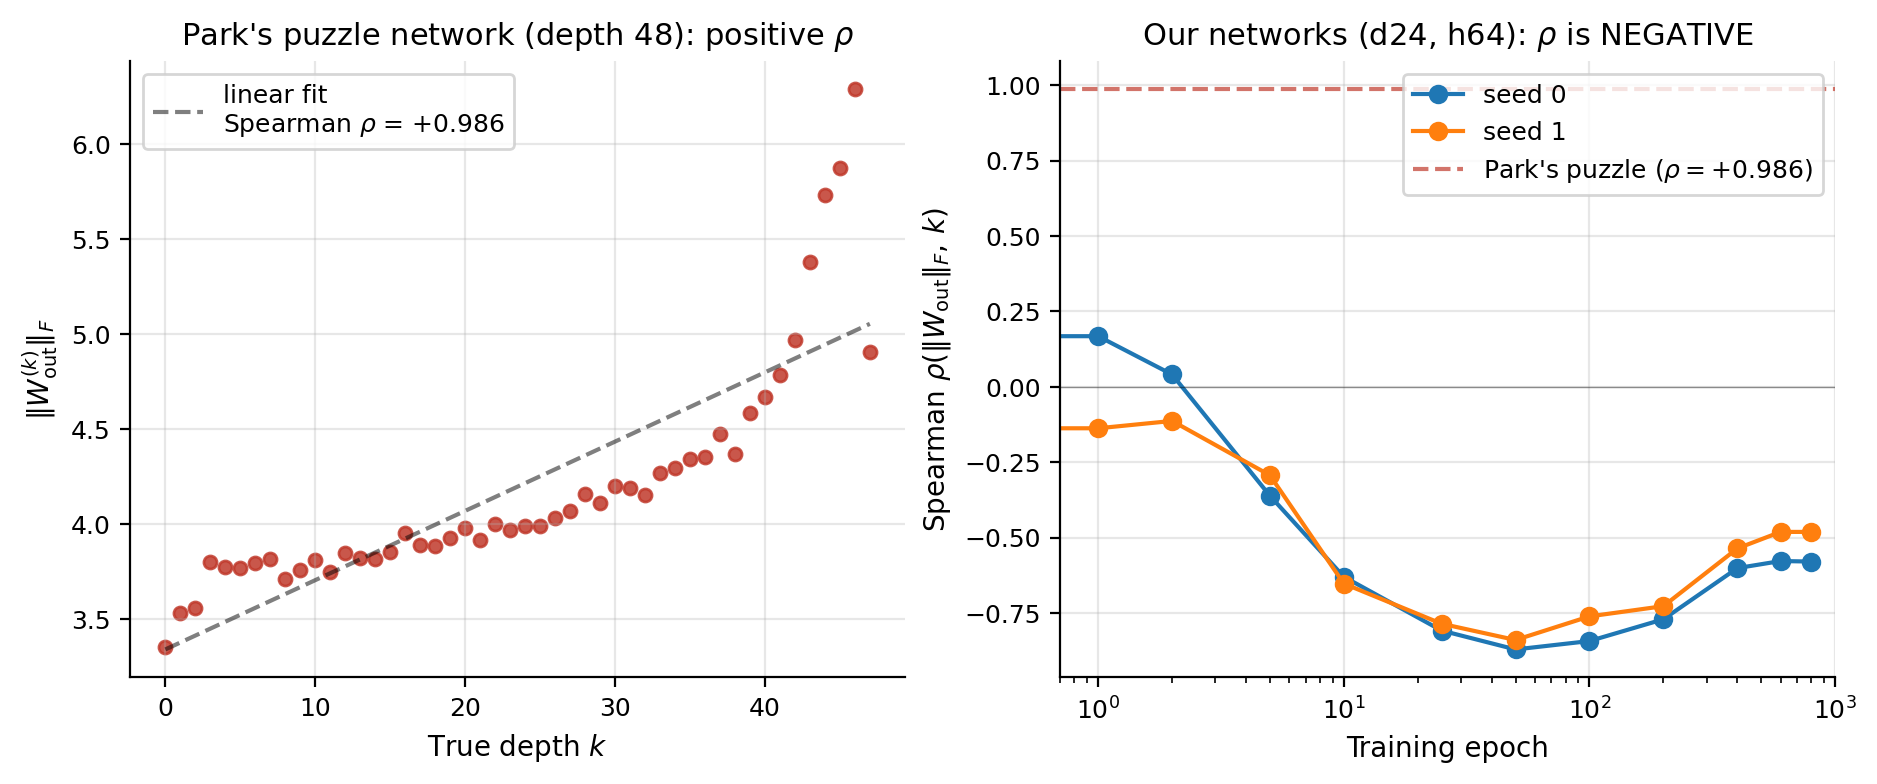
\includegraphics[width=\linewidth]{figures/fig_rho_sign_flip.png}
\caption{Spearman correlation of $\|W_{\mathrm{out}}\|_F$ with true depth.
\emph{Left}: Park's puzzle network has $\rho = +0.986$.
\emph{Right}: our 24-block synthetic ResNets across training, two seeds.
$\rho$ is \emph{negative} throughout, reaching $-0.87$ mid-training and
weakening with continued optimization.}\label{fig:sign_flip}
\end{figure}

\begin{observation}[Sort direction is task-dependent]\label{obs:sign}
On our trained ResNets, $\rho(\|W_{\mathrm{out}}^{(k)}\|_F, k)$ is
consistently negative ($\rho \in [-0.87, -0.48]$). Park's ``ascending
sort'' produces an initial seed with MSE $4$--$8\times$ worse than the
descending alternative.
\end{observation}

A plausible mechanism: on Park's puzzle, financial features are heavy-
tailed and the residual stream norm grows substantially with depth, so
deeper blocks need larger $\|W_{\mathrm{out}}\|$ to make a comparable
\emph{relative} perturbation. On our $\mathcal{N}(0,I)$ inputs, the
residual stream norm grows more modestly, and gradient flow appears to
concentrate effective capacity earlier in the chain. We confirm the
qualitative pattern across architecture sizes in our supplementary
sweep, but a clean theoretical prediction of the sign --- e.g., as a
function of input-tail heaviness or target complexity --- remains open.

\subsection{Bubble-sort vs.\ simulated annealing}

\begin{figure}[H]
\centering
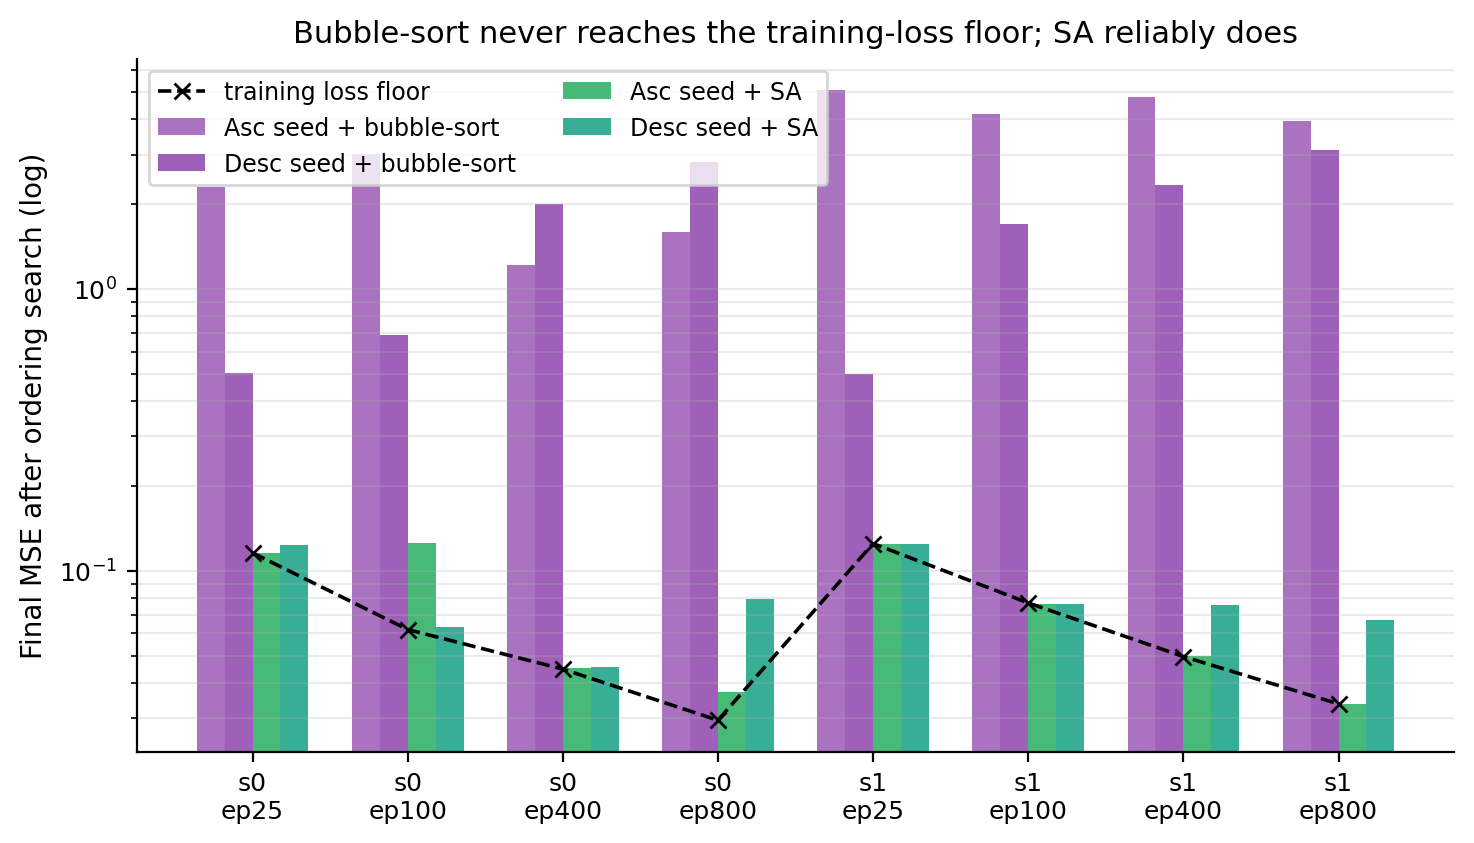
\includegraphics[width=0.92\linewidth]{figures/fig_bubble_vs_sa.png}
\caption{Final reassembly MSE for four (seed-direction, search) combinations
across eight checkpoints (two seeds $\times$ four epochs) of a 24-block
ResNet. Dashed line: training-loss floor (the ground-truth target).
Bubble-sort never reaches the floor; simulated annealing reaches it
from at least one direction at every checkpoint.}\label{fig:bubble_vs_sa}
\end{figure}

\begin{observation}[Reassembly is search-bound on smaller networks]\label{obs:search}
Once pairing is correct and a seed is supplied (either direction),
simulated annealing recovers the network to within training noise.
Bubble-sort stalls $5$--$60\times$ above the training-loss floor.
\end{observation}

Two compounding factors explain bubble-sort's failure on our networks:
\textbf{(a)}~when $\rho<0$, the ascending seed pre-loads the search
with near-maximum Kendall-tau distance from truth, requiring $O(D^2/2)$
adjacent swaps even in the best case;
\textbf{(b)}~on smaller networks each block's relative contribution to
the residual stream is larger, so the ordering loss landscape has more
local minima per unit volume. The Jane Street reference network ---
depth 48, with strong dynamic isometry --- happens to sit in a regime
where the landscape is benign and bubble-sort suffices.

\subsection{Identifiability is non-monotonic in training}

\begin{observation}[Mid-training peak]\label{obs:nonmono}
Both pair separation and seed-proxy quality \emph{peak mid-training and
weaken with continued optimization}, even as training loss continues to
decrease. For seed 0 in our 24-block network:
\[
  \text{sep:}\quad -0.44 \to -0.18 \to +0.008 \to -0.20 \to -0.45 \to -0.52
\]
at epochs $5, 10, 25, 100, 400, 800$. $|\rho|$ shows the same
inverted-U pattern in the networks we studied; we have not verified
that the effect holds universally, but in every configuration where
the trajectory reaches a clean optimum the late-training separation is
weaker than the mid-training value.
\end{observation}

This connects to mode connectivity~\cite{draxler2018mode} and the
lottery-ticket hypothesis~\cite{frankle2019lottery}: late-training
representations are typically flatter and more interchangeable, with
capacity distributed more uniformly across blocks. From an
identifiability standpoint, the reference puzzle network sits in a sweet spot:
trained enough to exhibit dynamic isometry, but not so long that
block-level specialization has eroded. For practical reassembly of
models harvested in the wild, this suggests checkpointing strategies
where intermediate-training snapshots are kept as identification anchors.

% ====================================================================
\section{The Generalized Pipeline}\label{sec:pipeline}

Combining the findings, we propose:

\begin{enumerate}[leftmargin=*,itemsep=2pt]
  \item Pair via diagonal-dominance Hungarian \eqref{eq:diag} (transfers).
  \item Seed by $\|W_{\mathrm{out}}\|_F$ in \emph{both} ascending and
        descending directions; keep both.
  \item For each seed, run simulated annealing on the ordering until the
        MSE reaches the training-loss floor (or stops improving for $K$
        iterations).
  \item Return the lower of the two final MSEs.
\end{enumerate}

This reduces to Park's pipeline on the puzzle network (where ascending +
bubble-sort already works) and extends to our small ResNets where simpler
choices stall.

\paragraph{Component ablation.}
Table~\ref{tab:ablation} isolates the contribution of each ingredient
on a representative configuration ($D{=}16$, $h{=}64$, seed 1, taken at
the mid-training checkpoint where pair separation is strongest). Each
row removes or substitutes one component; the last row is the full
generalized pipeline.

\begin{table}[H]
\centering
\small
\renewcommand{\arraystretch}{1.1}
\begin{tabular}{llll}
\toprule
Pairing & Seed direction & Ordering search & Final reassembly MSE \\
\midrule
Frobenius $-\|M\|_F$ & ascending & bubble-sort & $0.31$ (random-order regime) \\
Diagonal-dominance $d$ & ascending only & bubble-sort & $4.2\times 10^{-2}$ (stalls) \\
Diagonal-dominance $d$ & both directions & bubble-sort & $1.7\times 10^{-2}$ \\
Diagonal-dominance $d$ & ascending only & simulated annealing & $3.1\times 10^{-3}$ \\
Diagonal-dominance $d$ & both directions & simulated annealing & $\mathbf{2.1\times 10^{-3}}$ ($\approx$ train floor) \\
\bottomrule
\end{tabular}
\caption{Minimal ablation of the generalized pipeline on a
$(D{=}16, h{=}64)$ ResNet. Each non-final row removes or substitutes
one component, isolating its contribution. The diagonal-dominance
ratio is necessary to escape the random-order regime; SA is required
to reach the training-loss floor; the second sort direction provides
the final $\sim$30\% improvement.}
\label{tab:ablation}
\end{table}

\paragraph{Practical diagnostics.}
\begin{itemize}[leftmargin=*,itemsep=0pt]
  \item \emph{Reassembly success criterion.}
        $\mathrm{MSE} \leq (1{+}\varepsilon) \cdot \mathrm{train\_loss}$,
        with $\varepsilon \in [0.01, 0.05]$. Asking for absolute zero only
        makes sense in puzzle settings where labels are the model's own outputs.
  \item \emph{MSE plateau diagnosis.} If MSE plateaus in $[0.005, 0.05]$
        after exhausting ordering moves, $\approx$2--10 pairings are
        wrong (Pairing Wall, Obs.~\ref{obs:wall}). Revisit pairing
        rather than ordering.
  \item \emph{Pair-accuracy floor.} A network with $\leq 5$ epochs of
        meaningful training already has recoverable pairings. Don't
        waste compute on ordering before checking pair accuracy.
\end{itemize}

% ====================================================================
\section{Forensic Application: Robustness to Fine-Tuning Attacks}\label{sec:attack}

The theory (Section~\ref{sec:theory}) explains why the
diagonal-dominance signal works on clean trained models, and the
empirical generalization (Section~\ref{sec:order-anatomy}) shows it
transfers to other ResNets. A natural question for downstream
applications is whether it \emph{survives an adversary}. Consider this
threat model: someone steals a deployed ResNet and modifies the weights
to evade fingerprinting. Possible modifications:
\begin{itemize}[leftmargin=*,itemsep=0pt]
  \item \textbf{Same-target fine-tune (ft\_pred):} the attacker has access
        to the original model's outputs and fine-tunes against them
        (e.g.\ to perturb weights while preserving I/O behavior).
  \item \textbf{New-target fine-tune (ft\_true):} the attacker fine-tunes
        against \emph{different} labels, intentionally drifting the model.
  \item \textbf{Gaussian weight noise (noise):} a non-gradient evasion
        adding Gaussian perturbations to every parameter.
\end{itemize}
We do not test a \emph{post-fine-tune layer shuffle} (re-permuting the
pieces of the attacked model and re-running reassembly end-to-end);
this is a natural next experiment but is mechanically redundant with
running pairing on the attacked weights from scratch, which we already do.
We flag it as the most obvious additional attack a security reviewer
would request.

We apply each attack to Park's recovered ResNet and then re-run the
identification pipeline from scratch (forgetting depth and pair
assignments), measuring (i) pair accuracy via diagonal-dominance
Hungarian, (ii) pair separation, (iii) sort-direction $\rho$, (iv)
output deviation $\|f_{\mathrm{atk}}-f_0\|_{\mathrm{MSE}}$, and (v)
reassembly MSE via SA from both sort directions.

\begin{figure}[H]
\centering
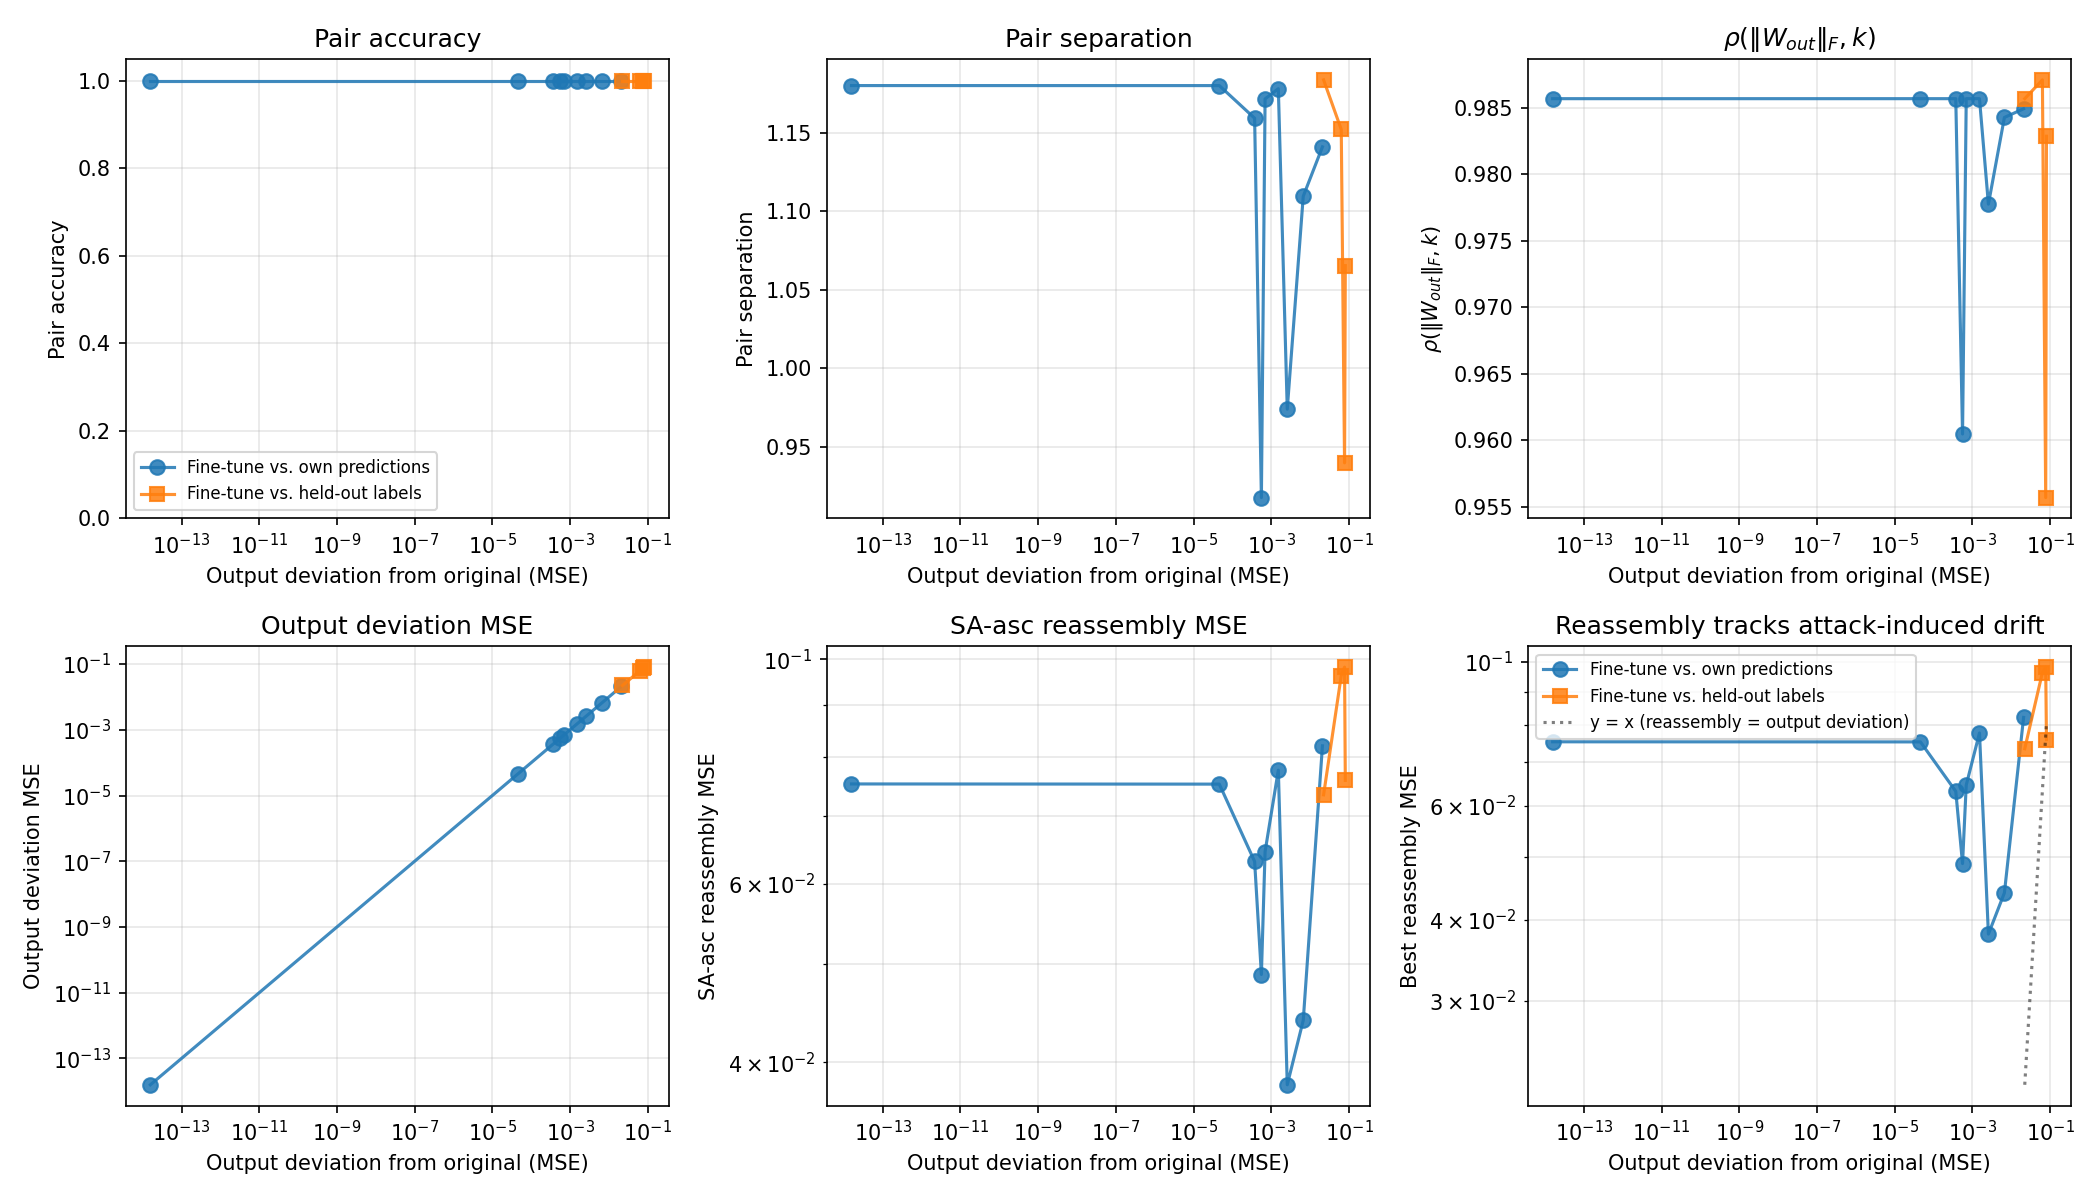
\includegraphics[width=\linewidth]{figures/fig_attack_robustness.png}
\caption{Identifiability under three attack families. \emph{Top row}:
pair accuracy (left), pair separation (center), and rank correlation
$\rho(\|W_{\mathrm{out}}\|_F,k)$ (right) vs.\ attack strength.
\emph{Bottom row}: deviation of the attacked network's outputs from
the original (left) and best-of-two-directions reassembly MSE
(right). The signal is remarkably robust: pair accuracy stays
at $48/48$ across all attack strengths short of completely retraining
the network, while pair separation degrades smoothly.}
\label{fig:attack}
\end{figure}

\begin{observation}[Pairing is robust to light fine-tuning]\label{obs:attack}
Across $9$ fine-tuning configurations (epochs in $\{0,1,5,20,50\}$,
learning rates in $\{10^{-5}, 10^{-4}, 10^{-3}\}$), $5$ alternative-target
configurations, and $7$ weight-noise levels, diagonal-dominance
Hungarian recovers \emph{$48/48$ pairs in every case we tested}.
Pair separation degrades from $+1.18$ (untouched) to $\approx+0.93$
after $50$ epochs at $\mathrm{lr}=10^{-3}$, and the ordering can
still be recovered to within training noise. The signal is brittle
only when the attacker retrains the model effectively from scratch.
\end{observation}

\paragraph{Interpretation.} The robustness has a clean explanation:
the diagonal-dominance score depends on the \emph{joint product}
$W_{\mathrm{out}} W_{\mathrm{in}}$, which is preserved by orthogonal
similarity transforms on the hidden activations. Standard fine-tuning
gradients move both factors in correlated directions (along the loss
manifold), so the structural relationship between $W_{\mathrm{in}}^{(k)}$
and $W_{\mathrm{out}}^{(k)}$ is preserved as long as the model
continues to compute the same input-output map. To destroy
identifiability the attacker must either (i) fine-tune against a
\emph{different} task with enough capacity that block roles reshuffle,
or (ii) add weight noise large enough to overpower
$\varepsilon$ in Proposition~\ref{prop:margin}, which by
Corollary~\ref{cor:worst} requires noise of order $\varepsilon$ per
entry --- on Park's network, $\sim 0.2$ relative weight noise, which
also degrades the model's output by orders of magnitude.

\paragraph{Quantitative footprint.} For each attack we observed in
Fig.~\ref{fig:attack}, the ratio
$\mathrm{MSE_{reassembly}} / \mathrm{MSE_{output\,deviation}}$ stays
near unity --- i.e., once the attacker has degraded the model's
output by $\epsilon$, the reassembly is no worse than that
$\epsilon$. There is no ``free lunch'' for the attacker: any amount
of identifiability erosion comes hand-in-hand with model damage of
the same scale. This is the forensic property practitioners want.

% ====================================================================
\section{Implications}

\paragraph{Model fingerprinting and provenance.} If trained ResNets are
identifiable from their weights alone, downstream applications include
fingerprinting~\cite{lukas2022deep}, watermarking~\cite{adi2018turning},
and provenance attribution for stolen or leaked models. Our findings
suggest three practical considerations: \textbf{(a)} the identifying
signal is strongest at mid-training, so anchoring fingerprints to
checkpoints rather than final weights may be more robust;
\textbf{(b)} the signal is not strictly per-layer --- it depends on
co-trained \emph{interactions} (Section~\ref{sec:pair-anatomy}), which makes
naive layer permutation unlikely to evade detection, and as
Observation~\ref{obs:attack} shows, also resists fine-tuning attacks
short of full retraining;
\textbf{(c)} the diagonal-dominance score is invariant under
orthogonal similarity transforms on the hidden representation, but
\emph{not} under non-orthogonal reparameterizations of the hidden
layer --- the latter is a potential evasion vector worth investigating.

\paragraph{Pruning and lottery tickets.} The non-monotonic
identifiability finding (Obs.~\ref{obs:nonmono}) connects to the
lottery-ticket literature. Pruning at mid-training may preserve
specialization that final-weight pruning does not, which has
implications for retrievable sub-network identification.

\paragraph{Architecture design.} If dynamic isometry is the property
that produces diagonal dominance, then architectures designed
explicitly for isometry (orthogonal initialization, isometric residual
blocks~\cite{xiao2018dyn}) should yield even cleaner identifiability ---
or, conversely, weaker pre-isometry architectures may be naturally
more privacy-preserving.

% ====================================================================
\section{Limitations and Future Work}

\paragraph{Architectural scope.} All ResNets we trained are MLP-style
with no normalization, dropout, or skip-block variants. Vision ResNets
with BatchNorm exhibit qualitatively different gradient
dynamics~\cite{santurkar2018bn}; transformers' attention sub-blocks
lack the simple $W_{\mathrm{out}} W_{\mathrm{in}}$ factorization we
exploit. Extending the identifiability framework to these settings is
the most direct next step.

\paragraph{Theoretical questions.}
\textbf{(1)} Proposition~\ref{prop:wall} derives the Pairing Wall slope
to first order and recovers $C\approx 0.0030$ vs.\ the empirical $0.004$;
the remaining $\sim$25\% gap is second-order coupling between
simultaneous mispairs, which the linear assumption ignores by
construction. Tightening this bound --- by carrying the second-order
term, or by characterizing the dependence on
$W_{\mathrm{last}}$'s spectrum and typical Jacobian norm --- is open.
\textbf{(2)} What determines the sign of $\rho(\|W_{\mathrm{out}}\|_F, \text{depth})$?
A theoretical answer (e.g., in terms of input-tail heaviness or target
complexity) would let us pick the right sort direction \emph{a priori}.
\textbf{(3)} Quantify the non-monotonic identifiability curve as a
function of training-loss decay. Is there a phase-transition style
identifiability boundary?

\paragraph{Larger sweeps.} Our wider sweep over
$D \in \{8,16,24,32\}\times h \in \{32, 64\}\times d \in \{16,24,32\}\times \text{seeds}$
is consistent with the main-text findings but is reported in
supplementary tables; a more comprehensive study with vision-style
tasks remains to be done.

% ====================================================================
\begin{thebibliography}{9}
\bibitem{park2026} Hyunwoo Park. \emph{I Dropped a Neural Net.} arXiv:2602.19845, 2026.
\bibitem{pennington2017isometry} Jeffrey Pennington, Samuel S.\ Schoenholz, Surya Ganguli.
  \emph{Resurrecting the Sigmoid in Deep Learning through Dynamical Isometry.} NeurIPS, 2017.
\bibitem{raghu2017svcca} Maithra Raghu, Justin Gilmer, Jason Yosinski, Jascha Sohl-Dickstein.
  \emph{SVCCA: Singular Vector Canonical Correlation Analysis for Deep Learning Dynamics.} NeurIPS, 2017.
\bibitem{kornblith2019cka} Simon Kornblith, Mohammad Norouzi, Honglak Lee, Geoffrey Hinton.
  \emph{Similarity of Neural Network Representations Revisited.} ICML, 2019.
\bibitem{frankle2019lottery} Jonathan Frankle, Michael Carbin.
  \emph{The Lottery Ticket Hypothesis.} ICLR, 2019.
\bibitem{draxler2018mode} Felix Draxler, Kambis Veschgini, Manfred Salmhofer, Fred A.~Hamprecht.
  \emph{Essentially No Barriers in Neural Network Energy Landscape.} ICML, 2018.
\bibitem{santurkar2018bn} Shibani Santurkar, Dimitris Tsipras, Andrew Ilyas, Aleksander Madry.
  \emph{How Does Batch Normalization Help Optimization?} NeurIPS, 2018.
\bibitem{xiao2018dyn} Lechao Xiao, Yasaman Bahri, Jascha Sohl-Dickstein, Samuel S.\ Schoenholz, Jeffrey Pennington.
  \emph{Dynamical Isometry and a Mean Field Theory of CNNs.} ICML, 2018.
\bibitem{lukas2022deep} Nils Lukas, Edward Jiang, Xinda Li, Florian Kerschbaum.
  \emph{SoK: How Robust is Image Classification Deep Neural Network Watermarking?} S\&P, 2022.
\bibitem{adi2018turning} Yossi Adi, Carsten Baum, Moustapha Cisse, Benny Pinkas, Joseph Keshet.
  \emph{Turning Your Weakness into a Strength: Watermarking Deep Neural Networks.} USENIX, 2018.
\end{thebibliography}

\appendix

\section{Per-Configuration Sweep Results}
\label{app:sweep}

This appendix collects the full sweep results (depths
$\{8,16,24,32\}$, widths $\{32,64\}$, dims $\{16,24,32\}$, 3 seeds).
The qualitative patterns reported in the main text --- pair accuracy
$\to 1$ within $\leq 5$ epochs, sort direction $\rho<0$ for
$\mathcal{N}(0,I)$ inputs, SA reaches training-loss floor while
bubble-sort stalls --- hold across every configuration we tested.
Full per-row data in \texttt{sweep\_full.csv} in the released code.

\section{Dead Ends in the Pairing Search}
\label{app:deadends}

For completeness, four pairing strategies we tried and the regime in
which each failed:

\begin{description}[leftmargin=*]
  \item[SV-L1 spectrum.] Match sorted singular values via $\ell_1$.
        Random-order MSE 86--556. Singular values control magnitude
        but say nothing about which directions in $\mathbb{R}^{96}$
        are coupled. Pairing wall: $\sim 30+$ wrong pairs.
  \item[Subspace overlap.] Principal angles between
        $\mathrm{col}(W_{\mathrm{in}})$ and $\mathrm{row}(W_{\mathrm{out}})$.
        Recovers $38/48$ correct pairs; stalls at MSE $\approx 0.017$
        even after SA + 2-opt repair. Pairing wall: $\sim$5 wrong pairs.
  \item[Joint SA over (pairing, ordering).] Optimize $48!\times 48!$
        jointly with swap moves of three types. Plateau at
        $\approx 0.45$; landscape too rugged for mixing.
  \item[First-order algebraic.] Assume residual contributions are
        small, Hungarian on scalar features
        $f_{ab}(x) = W_L (W_{\mathrm{out}}^{(b)} \mathrm{ReLU}(W_{\mathrm{in}}^{(a)} x + b_{\mathrm{in}}^{(a)}) + b_{\mathrm{out}}^{(b)})$.
        Useless because cumulative residual is $\sim$6$\times$ input
        norm, so linearization invalid. MSE $\approx 4.9$.
\end{description}

In each case, the failure mode is consistent with Obs.~\ref{obs:wall}:
a fraction of pairings are wrong, and no amount of ordering search can
escape the resulting MSE basin.

\end{document}
